% ----------------------------------------------------
% Overall System Architecture
% ----------------------------------------------------
\documentclass[class=report,11pt,crop=false]{standalone}
\input{../Style/ChapterStyle.tex}
\makenoidxglossaries

\newacronym{fm}{FM}{frequency modulation}
\newacronym{lora}{LoRa}{Long Range}
\newacronym{iot}{IOT}{Internet of Things}
\newacronym{fsk}{FSK}{Frequency Shift Keying}
\newacronym{chirp}{CHIRP}{Compressed High Intensity Radar Pulse}
\newacronym{atps}{ATPs}{Acceptance Test Protocols}
\newacronym{hal}{HAL}{Hardware Abstraction Layer}
\newacronym{oled}{OLED}{Organic Light Emitting Diode}
\newacronym{rssi}{RSSI}{Received Signal Strength Index}
\newacronym{uart}{UART}{Universal Asynchronous Receive and Transmit}
\newacronym{usb}{USB}{Universal Serial Bus}
\newacronym{css}{CSS}{Chirp Spread Spectrum}
\newacronym{i2c}{I2C}{Inter-Integrated Circuit}
\newacronym{spi}{SPI}{Serial Peripheral Interface}
\newacronym{gps}{GPS}{Global Positioning System}
\newacronym{nmea}{NMEA}{National Marine Electronics Association}
\newacronym{mac}{MAC}{Media Access Control}
\newacronym{sf}{SF}{Spreading Factor}
\newacronym{arr}{ARR}{Auto Reload Register}
\newacronym{sdr}{SDR}{Software Defined Radio}
\newacronym{pcb}{PCB}{Printed Circuit Board}
\newacronym{fdm}{FDM}{Frequency Division Multiplexing}


\newacronym{radar}{RADAR}{Radio Detection and Ranging}
\newacronym{ofdm}{OFDM}{Orthogonal Frequency Division Multiplexing}
\newacronym{tdm}{TDM}{Time Division Multiplexing}
\newacronym{tdma}{TDMA}{Time Division Multiple Access}
\newacronym{att}{AT\&T}{American Telephone and Telegraph Company}
\newacronym{usrp}{USRP}{Universal Software Radio Peripheral}
\newacronym{uct}{UCT}{University of Cape Town}


\begin{document}
% ----------------------------------------------------
\chapter{System Design \label{ch:systemdesign}}
% ----------------------------------------------------
Rory test be able to implement a LoRa-based communication system, the entire transmission and receive system had to be designed and built from scratch. The following chapter outlines the step-by-step process that went into the design of the transmission and receive modules of the overall system. The manner in which the design process was performed will be thoroughly outlined and discussed, and the benefits of each design decision will be discussed in detail.

To get an idea of exactly what parameters the overall system needs to adhere to, a requirement analysis needs to be performed.

\section{Requirement Analysis}
\subsection{Overall System Requirements}\label{subsec:systemreqs}
The following are the base requirements for the overall system that are derived from the project briefing.

\begin{enumerate}
    \item The system must be able to transmit data at a bandwidth that is not too slow that it does not allow for packet transmission in intervals that are too small to be useful, nor must it be too fast that transmission distance is hindered by the choice of LoRa parameter settings.
    \item The transmission system must have the ability to transmit data over large enough distances that could conceivably be seen by a real-world radiosonde module. This includes horizontal and vertical transmission distances.
    \item The system must be able to handle the extreme temperatures that may be experienced at higher altitudes by the radiosonde module.
\end{enumerate}

\subsection{Overall System Specifications}\label{subsec:systemspecs}
Based on the requirements listed above, a set of numerical based specifications for the overall system can be produced. These can be seen below.
\begin{enumerate}
    \item The system must have a bandrate of between 1200 bits/s and 4800 bits/s. 
    \item The system must have a range of 100km. 
    \item The system must be able to operate consistently at an altitude of 35km to 38 km.
    \item The system needs to be able to operate down to a temperature of -90\textdegree C\footnote{This requirement has been changed to roughly -40\textdegree C, due to there being an allowance for internal heating of the system.}.
\end{enumerate}

\subsection{Overall System Acceptance Test Protocols}
The following \gls{atps} were derived from the overall system requirements and specifications found in section \ref{subsec:systemreqs} and \ref{subsec:systemspecs} respectively. 
\begin{enumerate}
    \item The bandrate of the system must be determined by performing an analysis to calculate the exact bandrate that the LoRa module is operating within based on the current parameters that the LoRa module is programmed with. This must be between the specified bandrate values mentioned in section \ref{subsec:systemspecs}.
    \item The range of the system must be maximised. To maximise the range, tests must be performed to determine the exact parameters that allow for the best transmission range. To pass this ATP, the specific combination of parameters that have been determined to maximise transmission range needs to allow for communication distances of around the specified 100km.
    \item The combination of components in the various modules need to all be able to handle temperatures down to as low as -40\textdegree C. This can be primarily determined from datasheets.
\end{enumerate}

\section{Modules and Sub-modules}
To aid in the ease of the design process, and to make the design of the overall system more manageable, the hardware for the entire system was split up into respective "black boxes". These black boxes make designing, building, and testing a more manageable task because they allow the larger problem to be broken up into smaller chunks. This way of thinking is analogous to modules and sub-modules, or systems and sub-systems. This method of design is excellent in that it allows the designer to break a problem into smaller and smaller chunks, and as mentioned before, this makes a big problem more manageable.

The overall system can be broken up into two main sub-modules, these are the transmit module and the receive module. This is pictured in figure \ref{fig:overallModules} below.

\begin{figure}[H]
    \centering
    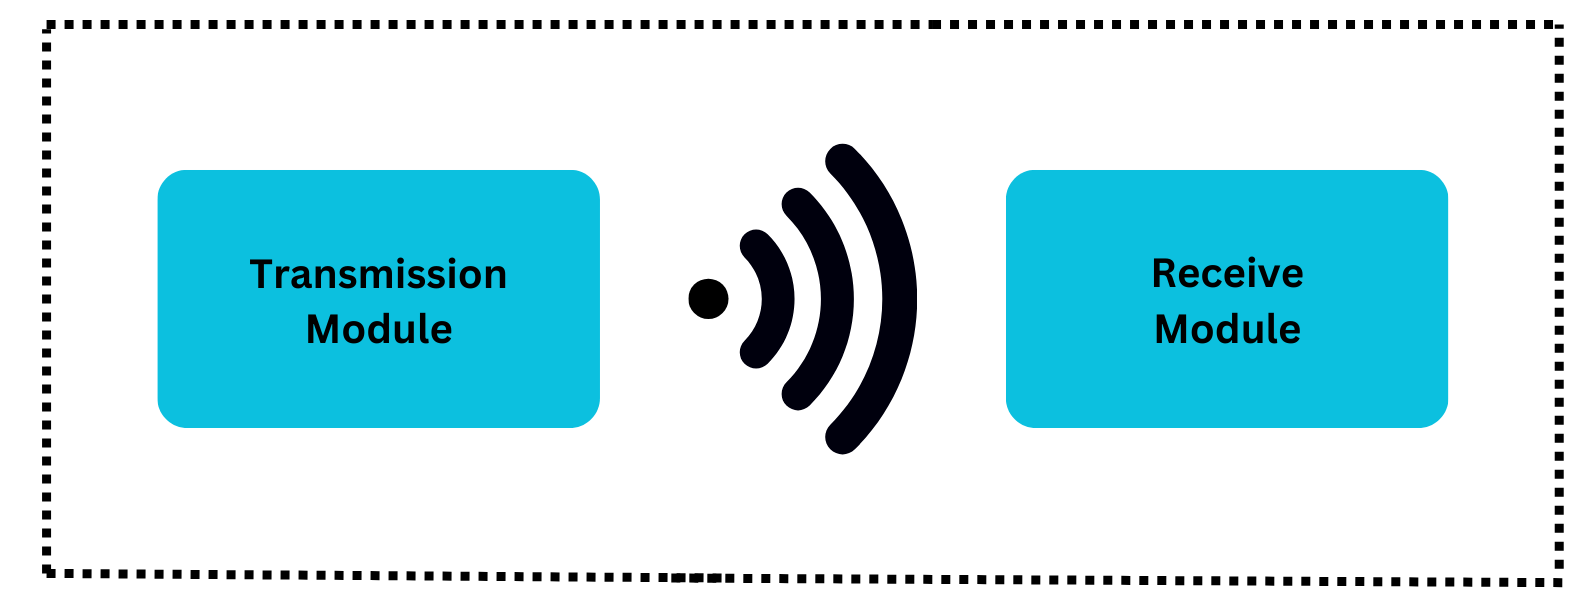
\includegraphics[width=0.7\linewidth]{../Images/overallModules.png}
    \caption{Overall module design of entire system}
    \label{fig:overallModules}
\end{figure}

The next step in the design process was to choose the specific components for the transmission and receiving circuits. The exact design thinking that went into the choice of components for each module is outlined in the following sections.

\section{Transmission Module Component Selection}
Continuing on with the module and sub-module method of design, the transmission system can be broken into the following sub-modules.
\begin{enumerate}
    \item \textbf{The Power Circuitry}: This will supply all the power to the module and will include a battery and a charging circuit. 
    \item \textbf{The Microcontroller Unit}: This will perform any data processing that needs to take place, and will manage all the communication that needs to happen between the various sub-modules.
    \item \textbf{Sensor Module}: This includes all of the important sensors that take measurements and the various communication pathways to each sensor. 
    \item \textbf{The LoRa Module}: This module is responsible for anything to do with the transmission of messages using the LoRa communication protocol. 
    \item \textbf{The Display Module}: This module is responsible for displaying information to the user. This is especially important for the testing of the system. This testing procedure is described later on in chapter \ref{ch:methodology}.
\end{enumerate}

These sub-modules, as described above, are outlined in figure \ref{fig:transmissionModule} below.

\begin{figure}[H]
    \centering
    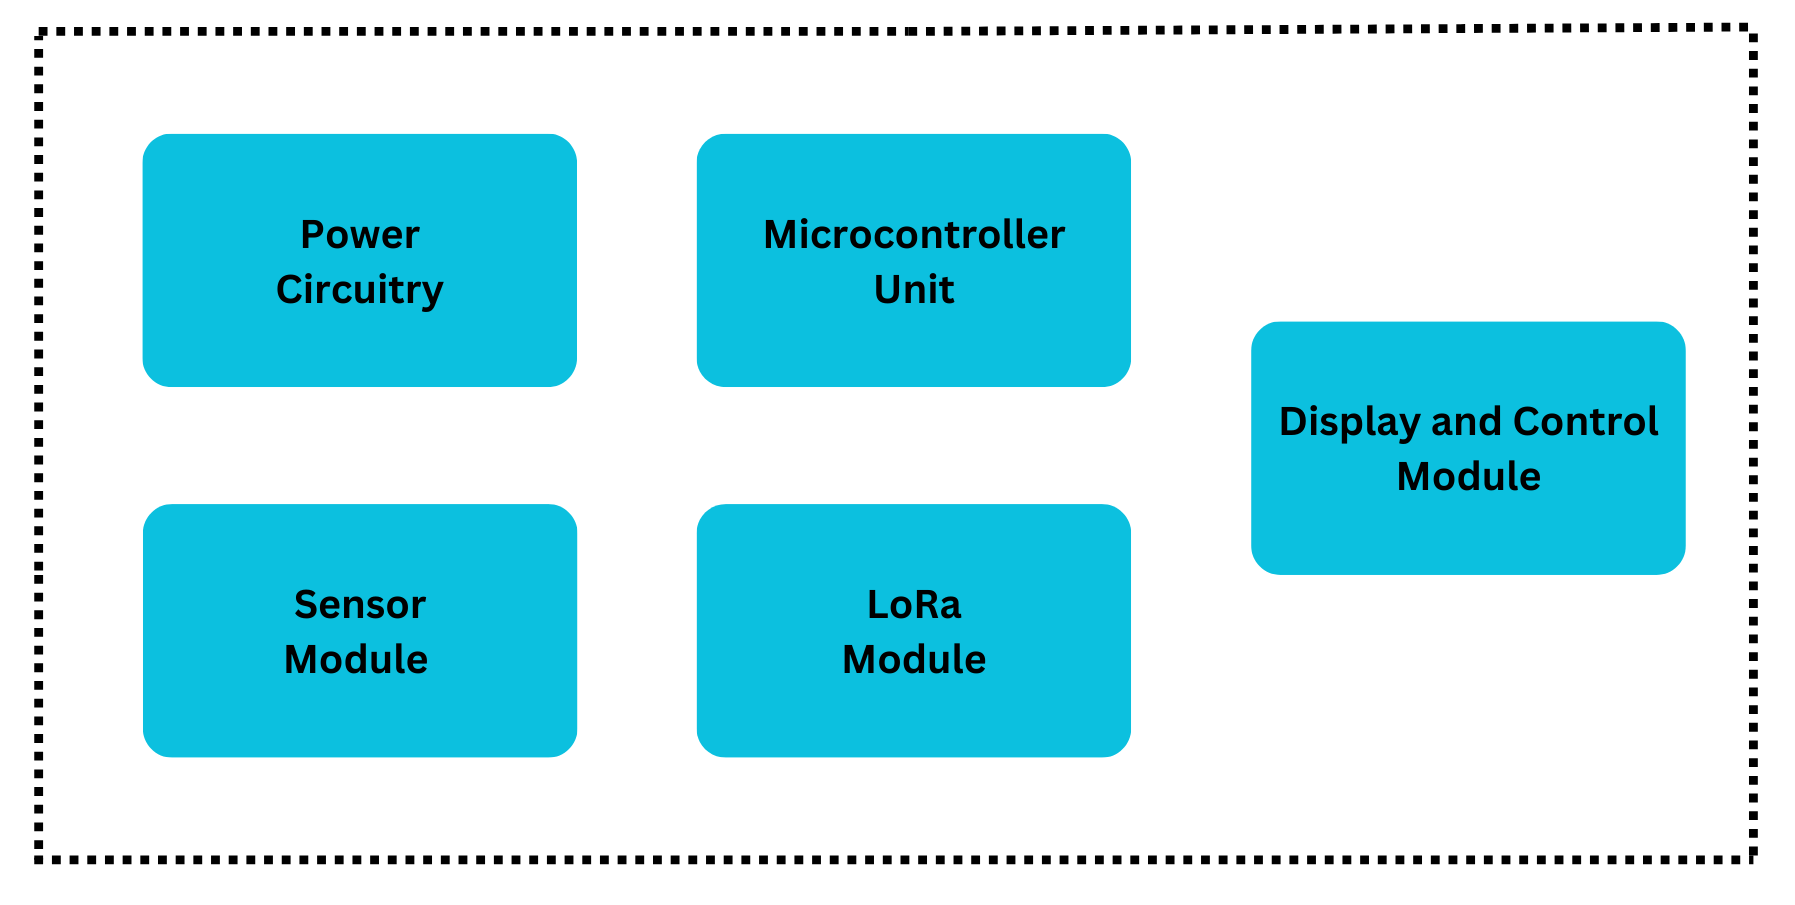
\includegraphics[width=0.7\linewidth]{../Images/transmissionModule.png}
    \caption{Overview of Transmission Module}
    \label{fig:transmissionModule}
\end{figure}

These various sub-modules each have their own design considerations and unique decisions which are outlined in the following sections.


\subsection{Microcontroller Unit}\label{sec:microcontrollerunit}
Various microcontrollers were considered for use in the transmission system. After some consideration, it was determined that the microcontroller unit had the following requirements.
\begin{enumerate}
    \item The microcontroller should be as low power as is viable for a transmission system such as this, due to the size and weight constraints of the device itself meaning that there is not a huge amount of battery capacity available.
    \item The microcontroller should have all the necessary communication protocols available to be able to communicate with the various sensor modules that will be implemented, for example, \gls{i2c}, \gls{spi}, and \gls{uart}.
    \item The microcontroller needs to be able to process packets of data from the various sensors that are available to it and must be able to create a single packet of data. Essentially it must be able to perform string processing based on the needs of the user.
\end{enumerate}

Of all the available options for microcontrollers in industry, the options were narrowed down to the following based on availability and previous personal experience with regards to working with the hardware. Firstly a simple Arduino Uno was considered. An Arduino Uno would have allowed for easy prototyping, since the Arduino framework for programming the boards is very well defined and user friendly, however, the Arduino itself is fairly large and doesn't have enough functionality. The very general specifications for the Arduino Uno are listed below in table \ref{tab:arduinounospecs}.

\begin{table}[H]
\centering
\begin{tabular}{|c|c|}
\hline
Programmable GPIO Pins  & 14   \\ \hline
UART               & 1    \\ \hline
SPI                & 1    \\ \hline
I2C                & 1    \\ \hline
Power Draw at Idle & 65mA \\ \hline
Onboard Serial to USB & Yes \\ \hline
\end{tabular}
\caption{Arduino Uno Specifications \cite{uno_r3_|_arduino_documentation_2023} \cite{how_much_power_an_arduino_uses_2023}}
\label{tab:arduinounospecs}
\end{table}

As you can see, the number of GPIO pins is not quite favourable, and the high power draw at idle is especially worrying considering that the whole system is going to be powered by a battery pack. With regards to the communication lines, technically it is possible to have one SPI and I2C line for multiple SPI and I2C devices, however, for testing purposes, I wanted to make each individual sensor or peripheral have its own communication line, which would make debugging issues a lot easier because one would be able to pinpoint exactly which lines may have issues without getting confused as to which sensor may be causing the problem. Based on all these considerations, it was decided that the Arduino Uno would not be a good choice for the transmitter circuit.

The second microcontroller that was considered was an ESP32. This is a NodeMCU-based microcontroller that has built-in WIFI and Bluetooth capabilities. The specific model to which I would have had access is the ESP32-WROOM-32D. This board can also be programmed with the Arduino framework using the embedded software development toolchain called PlatformIO. This means that programming the ESP32 would be as easy as programming an Arduino. This ease of development makes a significant difference when working on large projects because small issues tend to get solved faster due to more support for issues from the hobbyist Arduino community. This speeds up initial development drastically. The overall specifications for the ESP32 can be seen in table \ref{tab:esp32wroom32dspecs} below.


\begin{table}[H]
\centering
\begin{tabular}{|c|c|}
\hline
Programmable GPIO Pins & 22   \\ \hline
UART                   & 3    \\ \hline
SPI                    & 3    \\ \hline
I2C                    & 2    \\ \hline
Power Draw at Idle     & 80mA \\ \hline
Onboard Serial to USB & Yes \\ \hline
\end{tabular}
\caption{ESP32 Wroom 32D Specifications \cite{esp32_pinout_reference:_which_gpio_pins_should_you_use?_2018} \cite{insight_into_esp32_sleep_modes_their_power_consumption_2023}}
\label{tab:esp32wroom32dspecs}
\end{table}



As you can see from the above table, the ESP32 is a much better contender for the microcontroller position of the transmitter circuit because it has more GPIO pins and more communication channels than the Arduino. While it does have a slightly higher current consumption at idle, it is not too much more, making the higher current draw not too big of an issue. Another useful thing about the ESP32 is that it contains an onboard serial to USB converter. This makes debugging easier because a separate circuit, such as the ever-so-popular FTDI adaptor, is not required to easily view serial output from your embedded system. 

The third and last microcontroller that was considered for the transmitter circuit was an STM32-based microcontroller. The exact model that was analysed was the STM32F411 microcontroller. The STM32-based microcontrollers are great for projects such as this one because they are generally low-powered and bare metal. What I mean by bare metal is that they give the user/programmer the unique ability to access register level settings, which has been optimized with the \gls{hal} that has been developed by ST Microelectronics themselves. Table \ref{tab:stm32f411specs} below describes the overall specifications of the STM32F411.

\begin{table}[H]
\centering
\begin{tabular}{|c|c|}
\hline
Programmable GPIO Pins & 32  \\ \hline
UART                   & 3   \\ \hline
SPI                    & 5   \\ \hline
I2C                    & 3   \\ \hline
Power Draw at Idle     & 3mA \\ \hline
\end{tabular}
\caption{STM32F411 Specifications \cite{STM32F411}}
\label{tab:stm32f411specs}
\end{table}

As you can see, the STM32F411 has many more programmable GPIO pins than the Arduino or ESP microcontroller. The STM also has more communication peripheral lines than the other microcontrollers, and crucially, has a current draw that is incredibly small compared to the other options at idle. One of the downsides however of the STM32F411 is that it does not have an internal debugger, this makes programming the module slightly more cumbersome than the Arduino or ESP due to the fact that you need an external debugger each time you program the board. In addition to not having a debugger module built-in, the STM32F411 microcontroller is primarily programmed using the C programming language, with various drivers, such as the HAL. This can also make development a little bit slower due to inexperience and the C programming language generally not being as user-friendly as C++, which the Arduino and ESP variants get programmed with.


From all this information about the various microcontrollers which I had available to me, it was decided that the best microcontroller for the transmission circuit would be the STM32F411, due to the large number of programmable GPIO pins in comparison to the Arduino and ESP32, and the plethora of communication lines available, and finally, the low power draw. The STM32F411 would be able to meet all the requirements listed at the beginning of section \ref{sec:microcontrollerunit} with ease. It was decided that even though there may be some hurdles along the way with development taking longer than expected, the advantages seen by using the STM32F411 would far outweigh the disadvantages that may arise from it being harder to work with in the development phase.

\subsection{Sensor Module}
As described earlier, sensors play a vital role in a radiosonde device, and the choice of sensors makes a big difference as to what data you can accurately collect with each launch of the weather balloon system. The transmission system was designed to emulate the real-world requirements that a radiosonde module would have to follow. This includes making sure that all the correct sensors are implemented that would usually be implemented on a radiosonde module. For most radiosonde modules, and as mentioned in chapter \ref{ch:Literature}, the most important sensors that have to be implemented on a radiosonde module are the following:
\begin{enumerate}
    \item \textbf{A GPS Module}: This is used for two specific reasons, number one, a GPS module allows us to collect precise location data of the radiosonde module, and number two, the GPS allows for very precise timing data. This is very important for the data being collected because timestamped data is more useful than non-timestamped data.
    \item \textbf{Temperature Sensor}: This is vital for a radiosonde because it is one of the most crucial measurements that need to be taken at various altitudes.
    \item \textbf{Humidity Sensor}: This is used to determine relative humidity.
    \item \textbf{Pressure Sensor}: A pressure sensor is one of the most vital components because it allows for the calculation of altitude, which is important because, in conjunction with the temperature and pressure sensors, it allows scientists to determine how the temperature, pressure, and humidity change with altitude.
\end{enumerate}

From the above-listed sensors, the altitude can be calculated. Therefore, with these four sensors, all the most crucial measurements can be taken that a meteorologist would possibly want from a weather balloon system.

Firstly a GPS module needed to be chosen that is suitable for the transmitter circuit. After much searching, the GPS module that was the best choice based on availability and cost was the uBlox NEO-6M. This is a versatile GPS module that features the high-performance uBlox 6 positioning engine. This compact architecture and power and memory options make NEO-6M modules ideal for battery-operated mobile devices with very strict cost and space constraints \cite{NEO_6M}. The GPS module was purchased as a breakout board version and came with a dedicated ceramic-based antenna. An image of the purchased module can be seen below in figure \ref{fig:NEO-6M}.

\begin{figure}[H]
    \centering
    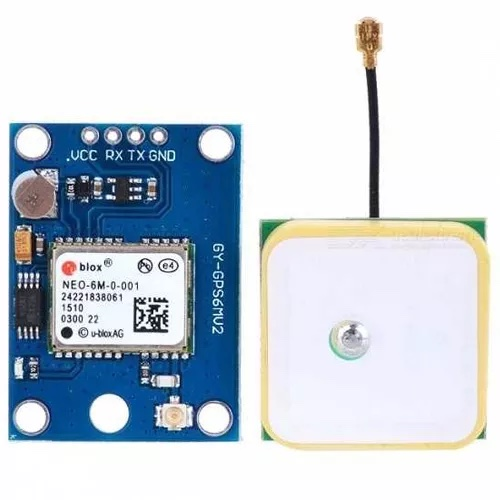
\includegraphics[width=0.4\linewidth]{../Images/NEO-6M.jpg}
    \caption{NEO-6M Gps Module}
    \label{fig:NEO-6M}
\end{figure}

Other than the already stated specification of the NEO-6M, the other features that the NEO-6M has can be seen in table \ref{tab:neo6mspecs} below.


\begin{table}[!ht]
    \centering
    \begin{tabular}{|c|c|}
    \hline
        \textbf{Receiver Type}: & 50 Channel GPS L1 frequency  \\ \hline
        \textbf{Time to First Fix}: &   \\ \hline
        Cold Start & 27s  \\ \hline
        Warm Start & 27s  \\ \hline
        Hot Start & 1s  \\ \hline
        Aided Start & <3s  \\ \hline
        \textbf{Sensitivity}: &   \\ \hline
        Tracking and Navigation & -161dBm  \\ \hline
        Reacquisition & -160dBm  \\ \hline
        Cold Start (without aiding) & -147dBm  \\ \hline
        Hot Start & -156dBm  \\ \hline
        \textbf{Maximum Navigation Update Rate}: & 5Hz  \\ \hline
        \textbf{Horizontal Position Accuracy}: & 2.5m  \\ \hline
        \textbf{Velocity Accuracy}: & 0.1m/s  \\ \hline
        \textbf{Heading Accuracy}: & 0.5 degrees  \\ \hline
        \textbf{Operational Limits}: &   \\ \hline
        Altitude & 50 000m  \\ \hline
        Velocity & 500m/s \\ \hline
    \end{tabular}
\caption{STM32F411 Specifications}
\label{tab:neo6mspecs}
\end{table}

Of particular note, is the hot start time. A hot start is when the GPS module remembers the last coordinate location when the device was turned on and tries to use this last stored location to quickly reconnect to the same satellites from before. This makes it very fast to get a GPS lock even when the device is turned on and off multiple times. This is particularly useful for testing purposes, as the device may be powered on and off multiple times per day for testing purposes. Considering all these features, it made sense to go with the NEO-6M as a GPS module for the transmission circuit.

The next sensors that needed to be implemented were the temperature, humidity, and pressure sensors. After much research, it was determined that a lot of the time you get multiple sensors that fall under the same category packaged into one module. Since temperature, humidity, and pressure all fall into the same category of atmospheric measurements, it was discovered that there exist many different options of sensor modules that incorporate all three into the same package. Of all these modules, I was recommended by a colleague to look into the BME280 designed and built by Bosch Sensortec.

The BME280 is a combined digital humidity, pressure, and temperature sensor. The fact that the module itself has three conjoined sensors within it makes for easier development than if three separate sensors were to be implemented one by one. This is because getting the correct drivers up and running for each device that you add to any embedded system takes a lot of time to do properly. The critical specifications of the BME280 module can be seen in table \ref{tab:bme280specs} below.

\begin{table}[H]
\centering
\begin{tabular}{|l|l|l}
\cline{1-2}
\textbf{Digital Interfaces}       & I2C and SPI                                                                               &  \\ \cline{1-2}
\textbf{Supply Voltage}           & 3.3V                                                                                      &  \\ \cline{1-2}
\textbf{Current Consumption}      & \begin{tabular}[c]{@{}l@{}}3.6uA @ 1Hz Humidity,\\ Pressure, and Temperature\end{tabular} &  \\ \cline{1-2}
\textbf{Operating Range}          &                                                                                           &  \\ \cline{1-2}
\multicolumn{1}{|c|}{Humidity}    & 0 - 100\% rel. Humidity                                                                   &  \\ \cline{1-2}
\multicolumn{1}{|c|}{Pressure}    & 30 000 - 110 000 Pa                                                                       &  \\ \cline{1-2}
\multicolumn{1}{|c|}{Temperature} & -40\textdegree C - 85\textdegree C                                                                                &  \\ \cline{1-2}
\end{tabular}
\caption{BME280 Specifications \cite{BME280}}
\label{tab:bme280specs}
\end{table}

Based on the above specifications, it was determined that the BME280 would make a perfect fit for the transmission module due to its combination of three separate sensors into one module, which would make development easier, its great power draw performance, and its brilliant operational ranges for humidity, pressure, and temperature. Much like the other modules, a breakout board version of the BME280 was purchased for ease of development and to make connecting it up to the prototype board easier, since the actual BME280 sensor comes in an extremely compact metal-lid LGA package with a footprint of only 2.5 x 2.5 mm$^{2}$ with a height of 0.93mm \cite{BME280}. An image of the purchased BME280 breakout module can be seen below in figure \ref{fig:bme280}.

\begin{figure}[H]
    \centering
    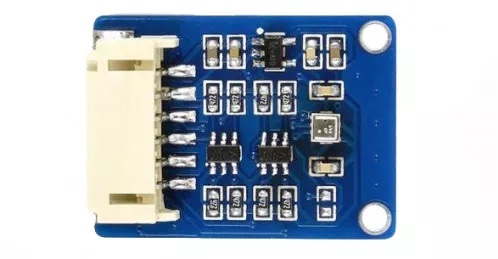
\includegraphics[width=0.5\linewidth]{../Images/BME280.jpg}
    \caption{BME280 Breakout Module}
    \label{fig:bme280}
\end{figure}

\subsection{LoRa Module}
The LoRa module is one of the most critical aspects of the entire transmission and receive systems. The requirements for the LoRa module are listed below.
\begin{enumerate}
    \item \textbf{Accessibility to Parameters}: It was vital that a LoRa module was chosen that gave the user access to the various LoRa modes available to the user. This is important because one of the main objectives of this prototype design is to determine which permutations of the LoRa parameters perform the best and therefore which parameters are best suited for use in a weather balloon radiosonde module.
    \item \textbf{Frequency Range}: The LoRa module needs to operate in the 433MHz range because the lower frequency operation mode allows for further transmission distances.
\end{enumerate}

Based on all this insight, I decided to look at a popular hobbyist LoRa module designed by Semtech with the product number SX1278. The SX1278 incorporates the LoRa spread spectrum modem which is capable of achieving a significantly longer range than existing systems based on FSK or OOK modulation and for maximum flexibility, the user may decide on the spread spectrum modulation bandwidth (BW), spreading factor (SF) and error correction rate (CR) \cite{SX1278}. The SX1278 was also the most widely available LoRa product on the South African market by far and was a reasonable price as well. The overall specifications of the LoRa module can be seen in table \ref{tab:sx1278specs} below.

\begin{table}[H]
\centering
\begin{tabular}{|l|l|}
\hline
\textbf{Frequency Range}               & 137MHz - 525MHz \\ \hline
\textbf{Spreading Factor}              & 6 - 12          \\ \hline
\textbf{Bandwidth}                     & 7.8kHz - 500kHz \\ \hline
\textbf{Supply Voltage}                & 3.3V            \\ \hline
\textbf{Operational Temperature Range} & -40\textdegree C - 85\textdegree C    \\ \hline
\textbf{Communication Protocol} & SPI \\ \hline
\end{tabular}
\caption{SX1278 Specifications \cite{SX1278}}
\label{tab:sx1278specs}
\end{table}

Much like the other modules used in the design, a breakout board was purchased that made the implementation of the LoRa module easier for prototype purposes. The exact module that was purchased can be seen below in figure \ref{fig:sx1278}.

\begin{figure}[H]
    \centering
    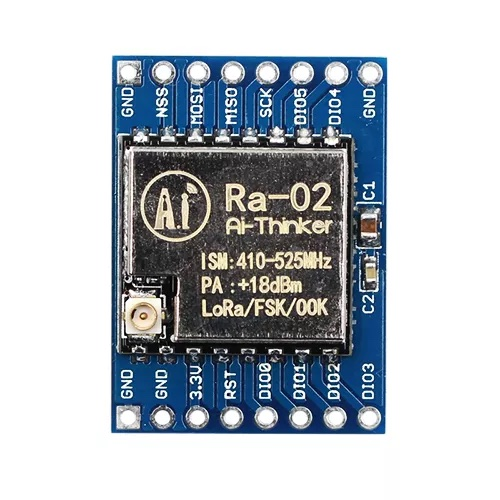
\includegraphics[width=0.4\linewidth]{../Images/SX1278.jpg}
    \caption{SX1278 Breakout Module}
    \label{fig:sx1278}
\end{figure}

This module includes a UFL connector which an antenna had to be purchased for. The choices of different antennae are vast and there are entire specialities that look into antenna design and fabrication however, for the purposes of easy initial testing, two different types of antenna were purchased. The two that were purchased were the simple dipole antenna, or "rubber duck" antenna, and the simple whip antenna. These different antennae can be seen in figure \ref{fig:variousantennae} below.

\begin{figure}[H]
\centering
\begin{subfigure}{.5\textwidth}
    \centering
    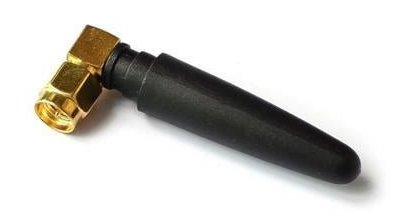
\includegraphics[width = 0.5\linewidth]{../Images/duck.jpg}
    \caption{"Rubber Duck" Antenna}
    \label{fig:duckantenna}
\end{subfigure}%
\begin{subfigure}{.5\textwidth}
    \centering
    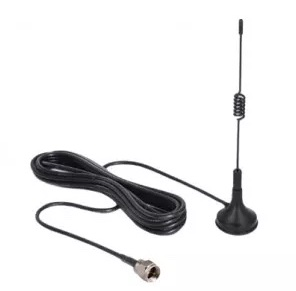
\includegraphics[width = 0.5\linewidth]{../Images/whip.jpg}
    \caption{Whip Antenna}
    \label{fig:whipantenna}
\end{subfigure}
\caption{Two Initial Antennae}
\label{fig:variousantennae}
\end{figure}

These two antennae are very good for testing purposes due to their low cost and ease of implementation into the overall system. It must be noted that different antennae sometimes use different connectors which can cause problems if not properly accounted for. For instance, the antennae that were purchased for this project have male SMA connectors, but the adaptor that was purchased to convert from the SMA at the antenna end to the UFL adaptor was a reverse polarity SMA. This caused issues and an appropriate adaptor had to be purchased. Following on from this, the overall specifications of the two different antennae can be seen in the tables in figure \ref{fig:variousantennaespecifications} below.




From these specifications, it can be seen that the whip antenna may perform slightly better than the duck antenna due to its higher antenna gain, and its higher output power capabilities. From initial inspection, the whip antenna is also slightly better than the "rubber duck" antenna because it comes with a 2m length of cable which makes placement of the antenna easier.

\subsection{Display and Control Module}\label{sec:displayandcontrolfortransmission}
The next module that had to have components purchased for it was the display and control module. The purpose of the display and control module was to give the user of the overall system a view into the exact mode that the system was on. It is important for the user to be able to see exactly what modes the device is on, as the various modes refer to what permutation of LoRa settings the device is currently using. The display and control module therefore has the following requirements.
\begin{enumerate}
    \item \textbf{Display of Mode}: It must be able to show the user of the system real-time information on the current system LoRa settings.
    \item \textbf{Control}: This module must give the user the ability to interact with the settings of the LoRa module and be able to manipulate and change the settings according to a predefined list of available modes.
\end{enumerate}

It was important that the display and control module were kept as simple as possible, to make the use of the overall device itself as easy as possible. The easier the device was to use, the easier it would be to do proper testing because the whole process would hopefully be smooth, especially with a well-designed interface. It was therefore decided that an \gls{oled} display would be used to display information about the system, with simple push buttons being implemented as a control mechanism to interface with the microcontroller unit of the transmission module. The OLED module that was chosen for the project was the SSD1306 powered module with a resolution of 128 x 64. The SSD1306 is a very popular driver chip for OLED modules and has lots of driver code available for free use and modification. The push buttons utilised were the simple momentary tactile push button switches widely available at various electronics stores. The exact modules purchased can be seen in figure \ref{fig:oledandpushbuttons} below.

\begin{figure}[H]
\centering
\begin{subfigure}{.5\textwidth}
    \centering
    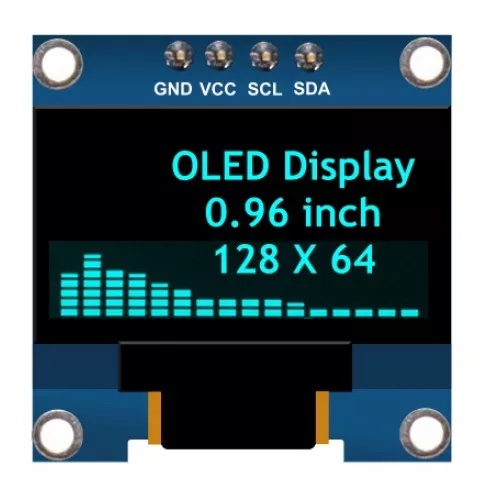
\includegraphics[width = 0.5\linewidth]{../Images/OLED.jpg}
    \caption{OLED Display}
    \label{fig:oleddisplay}
\end{subfigure}%
\begin{subfigure}{.5\textwidth}
    \centering
    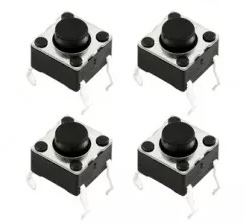
\includegraphics[width = 0.5\linewidth]{../Images/buttons.jpg}
    \caption{Momentary Push Button Switches}
    \label{fig:pushbuttonswitches}
\end{subfigure}
\caption{OLED Display and Push Button Switches}
\label{fig:oledandpushbuttons}
\end{figure}

The OLED display utilises the I2C communication protocol which the microcontroller controlling the transmission circuit has available. Using I2C for the OLED display also proved to be useful because it reduced the overall number of lines required which made building the prototype design more convenient, compared to using SPI, for example.

\subsection{Power Circuitry}\label{sec:powercircuitry}
As well as meeting all the overall system requirements, the power circuitry for the transmission system has the following requirements.
\begin{enumerate}
    \item \textbf{Power}: The power circuit must be able to supply the transmission circuit and all the peripheral devices that are a part of the transmission circuit with power at the correct voltage.
    \item \textbf{Battery Storage}: The power system should have a battery implemented to allow for wireless usage of the transmission system for testing purposes.
    \item \textbf{Battery Charging}: The power system must have a charging system in place for the battery, this charging system must be able to properly and safely charge the battery of choice.
\end{enumerate}


Many different circuit considerations were made, however, by far the easiest circuitry to implement given the stringent time frame of the project was a pre-built battery holder with charging and output circuitry built-in. This pre-built battery holder circuit can be seen below.

\begin{figure}[H]
    \centering
    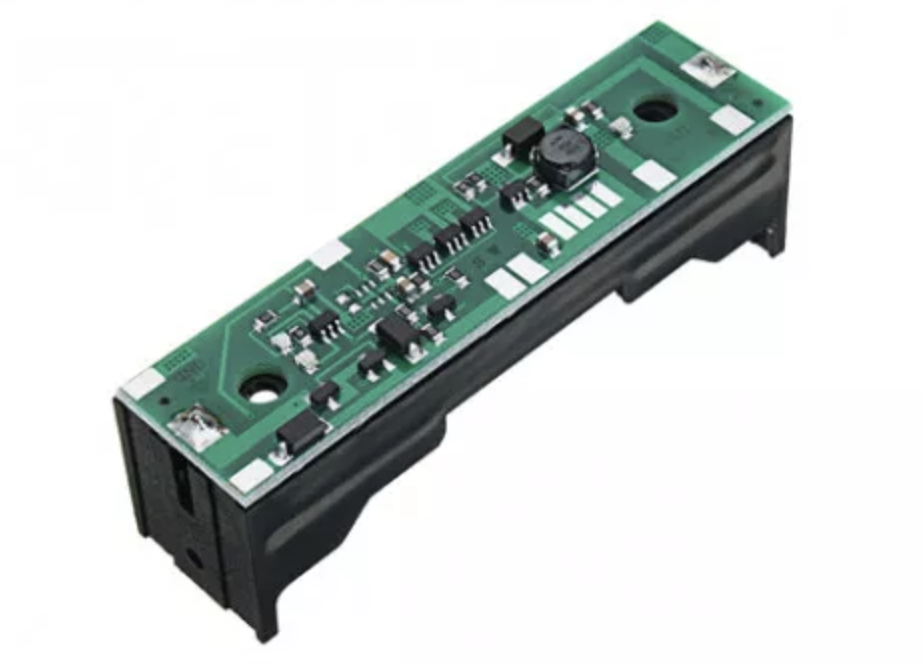
\includegraphics[width=0.5\linewidth]{../Images/batteryHolder.png}
    \caption{Selected Battery/Charging/Output Module}
    \label{fig:batteryHolder}
\end{figure}

One of the main reasons behind the choice of this particular power circuit was the fact that it had everything that the transmission circuit could need in a single package. Since the project was not about designing a power circuit, it also made a lot of sense to focus more time on other aspects of the project rather than designing custom power circuitry. 

This particular power circuit package is designed to hold an 18650 lithium ion battery. These batteries are very common and are great for projects exactly like this because they are durable and can deliver large amounts of power where necessary.

The electrical and physical characteristics of the power circuit are summarised in table \ref{tab:powercircspecs} below.

\begin{table}[H]
\centering
\begin{tabular}{|c|c|}
\hline
Input Charging Voltage         & 5.0V    \\ \hline
Regulated Output Voltage       & 5.0V    \\ \hline
Extended Period Current Output & 400.0mA \\ \hline
Extended Period Power Output   & 3.0W    \\ \hline
Length                         & 77.5mm  \\ \hline
Height                         & 23.1mm  \\ \hline
Width                          & 21.0mm  \\ \hline
Weight                         & 15.0g   \\ \hline
\end{tabular}
\caption{Table showing the power and physical characteristics of the power circuit}
\label{tab:powercircspecs}
\end{table}

In addition to the above figures in table \ref{tab:powercircspecs}, the power circuit also features overcharge protection, over-discharge protection, current limiting protection, over-temperature protection, and output short circuit protection. The small and lightweight nature of the battery holder is also a large advantage because the radiosonde system needs to be as small and lightweight as possible. 

\section{Receive Module Component Selection}
The receiving system is slightly simpler than the transmission module since it contains fewer components/sub-modules than the transmission system. With that being mentioned, the receive circuit can be broken up into the following sub-modules.

\begin{enumerate}
    \item \textbf{The Microcontroller Unit}: This unit will provide all the processing power to aid in the receiving of data packets from the LoRa module and must be able to perform the required string handling operations to display the received packets with relevant information about the packets themselves, such as the \gls{rssi}.
    \item \textbf{The Lora Module}: The LoRa module will connect to an external antenna and should be able to receive LoRa transmissions from the transmitter circuit. Much like the LoRa module on the transmission circuit, the LoRa module in the receiving circuit must have the ability to have programmable settings, such as the spreading factor and bandwidth.
    \item \textbf{The Power Module}: This module should be able to supply power to the entire receiver circuit. This circuit does not have to include a battery pack since it will connect to a computer for the recording of data. 
    \item \textbf{Display and Control Module}: This module is responsible for displaying the current LoRa settings to the user of the receiving circuit and it is responsible for giving the user the ability to change the current LoRa settings.
\end{enumerate}

Based on these above-mentioned submodules, an image of the broad system can be seen below in figure \ref{fig:receivemodule}. An overview of the selection process of the components contained within these modules will be discussed in the following sections.

\begin{figure}[H]
    \centering
    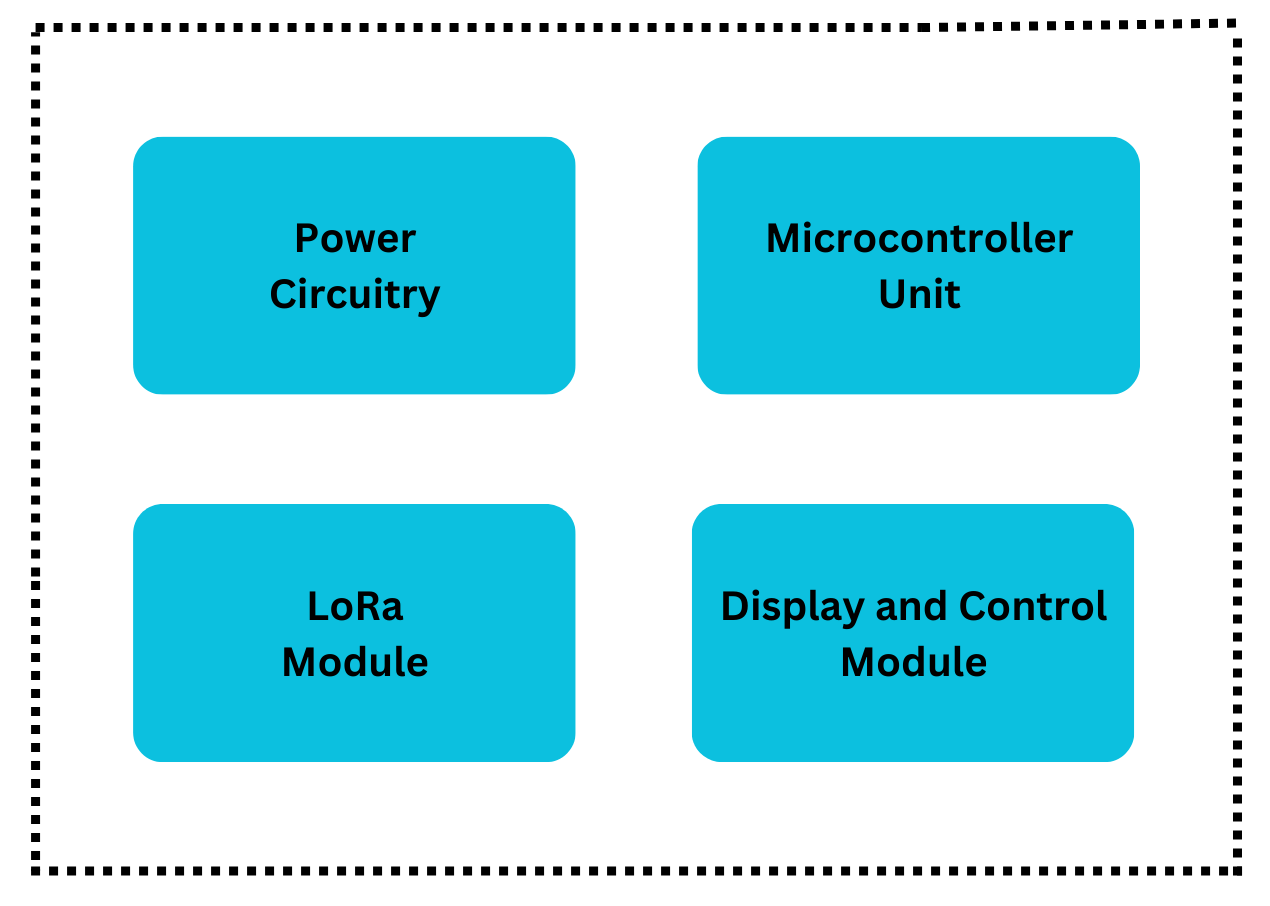
\includegraphics[width=0.6\linewidth]{../Images/receiveModule.png}
    \caption{Overview of the Receive Module}
    \label{fig:receivemodule}
\end{figure}


\subsection{The Microcontroller Unit}
The microcontroller choice is the biggest difference between the transmission and receiving circuits. Since the receiving circuit has to have the ability to easily output data to a computer, the choice of microcontroller choice differed from the microcontroller utilised in the transmission circuit. It was decided that the best and most efficient way to transfer data to the computer of the person using the system was via serial communication. Based on this, it would still be possible to use another STM32F411 as the microcontroller for the receiving system, however, the STM32F411 would require an external \gls{uart} to \gls{usb} convertor to be added to the circuit which would make the design more complex than necessary. It was therefore decided that the best option would be to use a microcontroller that has a built-in UART to USB converter. The main option for a device that has this capability and was readily available to me, was the ESP32-WROOM-32D board. This board was discussed in section \ref{sec:microcontrollerunit} however it was decided that it was not a good fit for the transmission module. This microcontroller is however a good option for the receiving module because it has a built-in UART to USB convertor, and it has more than enough GPIO pins to be able to handle all the needs of the receive module. This makes it a good fit for the receive module.

Another great aspect of using the onboard USB port of the ESP32-WROOM-32D board was that the ESP board itself could power the entire circuit. This made the design of the receive module more streamlined since an external power source did not have to be added. This meant that the power sub-module and the microcontroller unit were taken care of with one choice of microcontroller.

\subsection{LoRa Module}
For ease of component ordering and design, it was decided that the same LoRa module should be used in the receiving system as the transmission system. Therefore, the final choice of LoRa module for the receiving circuit was the SX1278 designed and manufactured by Semtech. The specifications of this specific module can be found in table \ref{tab:sx1278specs}. It makes sense to use the same LoRa module in the receive and transmit circuit because it ensures compatibility between the two modules. Sometimes different modules might have slightly different parameters due to the way in which they are produced. Using the same modules ensures that differences caused by design differences like this don't cause issues later on down the line. 

\subsection{Display and Control Module}
It was decided that the display and control module should be kept exactly the same as the transmission module. It was therefore decided that an OLED display would be used to display information about the system, with simple push buttons being implemented as a control mechanism to interface with the microcontroller unit of the receiver module. The OLED module and push buttons of choice are the exact same as for the transmission circuit and can be found in section \ref{sec:displayandcontrolfortransmission}.


\section{Hardware Interface Design}
The next step after the components for the transmission and receive modules were purchased, was to design and build prototype circuits for the two main sub-modules. The prototype circuits were built and tested using breadboards and 2.54mm stripboard. The breadboards were used to determine the exact workings of each module, for instance, the various sensors, before they were placed on the final stripboard prototype. Breadboards allow for quick and easy prototyping of circuits, however, they are fairly noisy due to the loose connections between components on them, and this is why stripboard is a better alternative to breadboards for semi-permanent prototypes.

\subsection{Transmission Module Interface Design}
The transmission module has many different interfaces between sub-modules that need to be connected in the correct way. A rough overview of the interfaces between the various sub-modules can be seen below in figure \ref{fig:transmissionmoduleinterfacing}.

\begin{figure}[H]
    \centering
    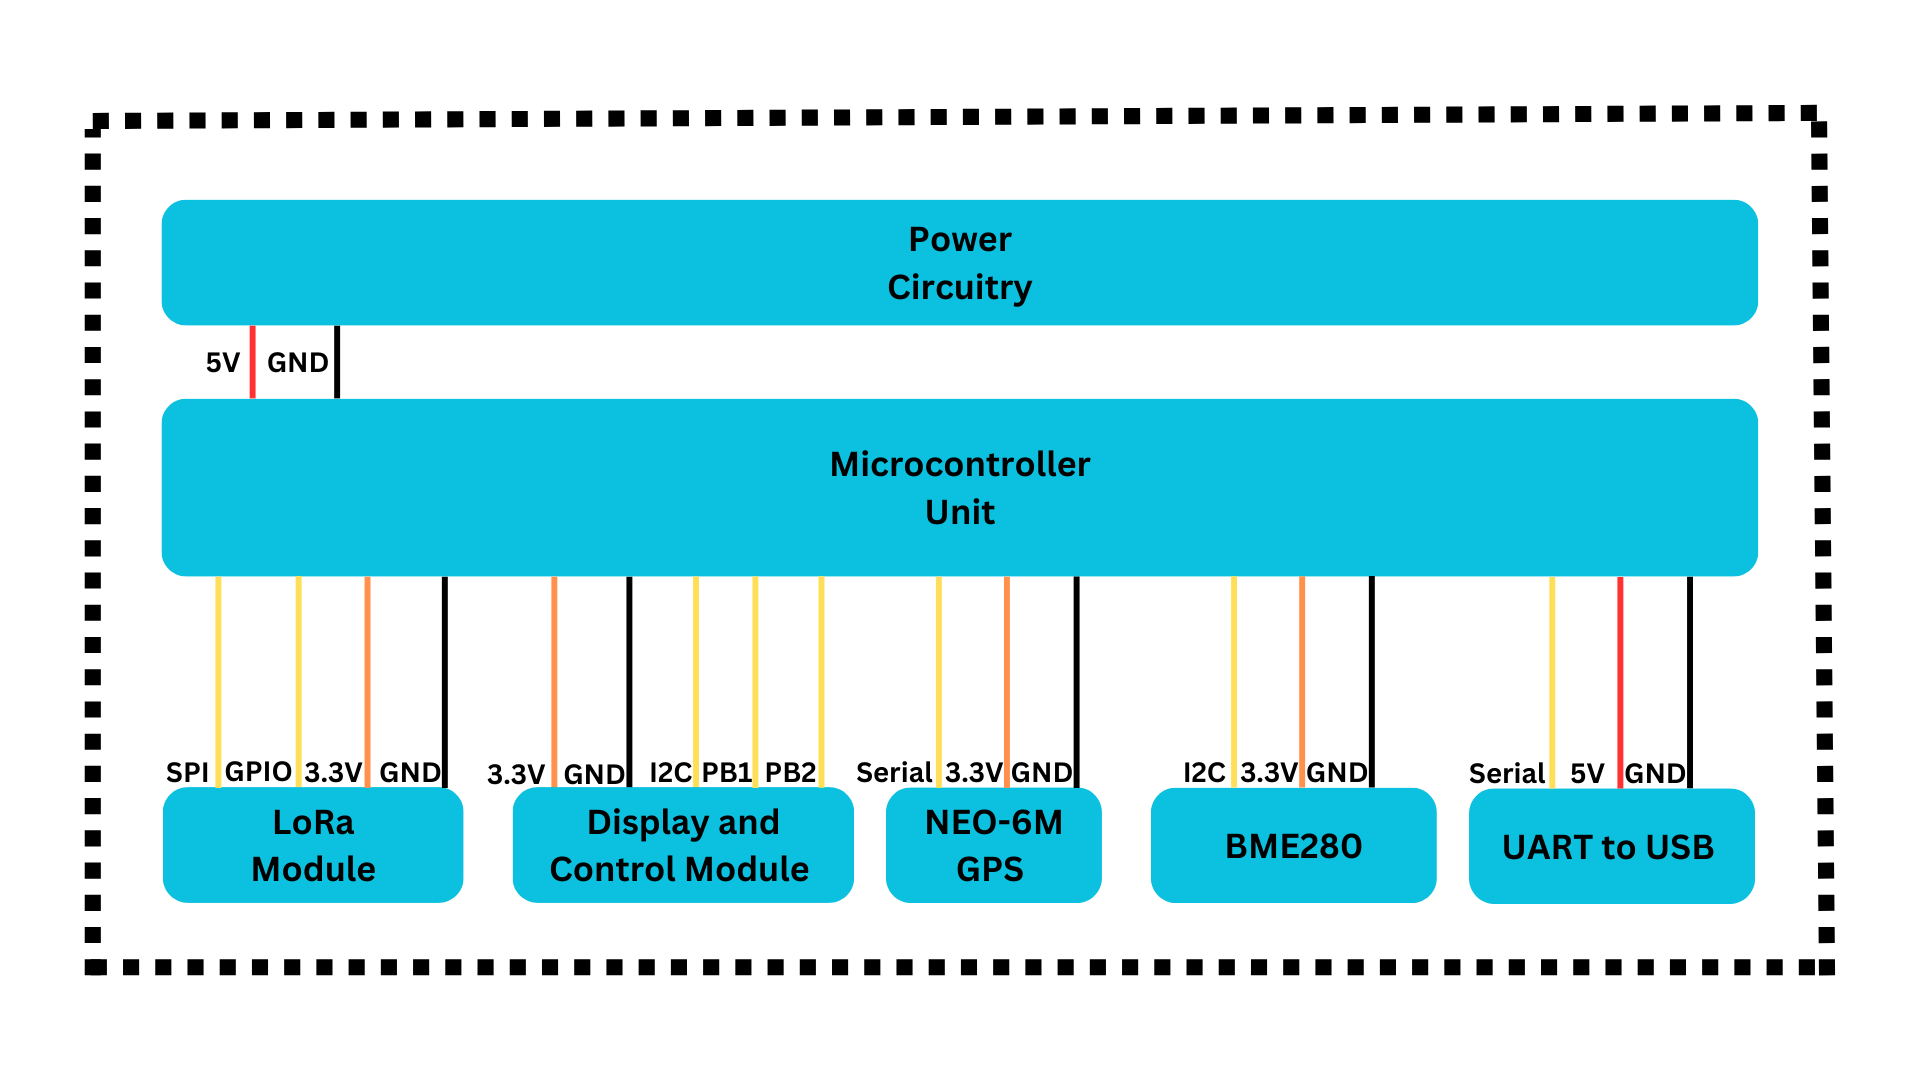
\includegraphics[width=0.8\linewidth]{../Images/transmissionModuleInterface.png}
    \caption{Overview of the Interfacing within the Transmission Module}
    \label{fig:transmissionmoduleinterfacing}
\end{figure}

As can be seen in the above figure, there are many different communication protocols in use. In fact, there are 2 I2C interfaces, 2 UART (serial) interfaces, and 1 SPI interface in use. As mentioned before, even though it is technically possible to run multiple devices off of one I2C or SPI communication link, for debugging purposes I made each individual device run on its own communication line, with no overlap of devices on the lines. This would make the design process easier due to the simple implementation of having individual devices on each communication line.

The portion of this broad outline which can be presented first is the microcontroller module. The full schematic for the microcontroller module can be seen below in figure \ref{fig:microcontrollermoduleschematic}.

\begin{figure}[H]
    \centering
    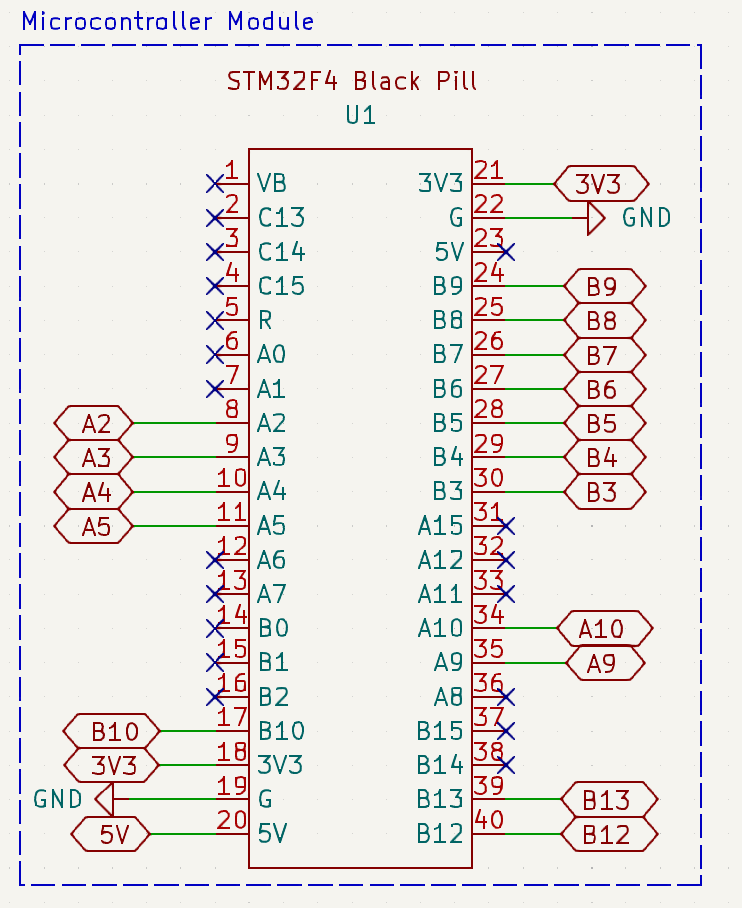
\includegraphics[width=0.45\linewidth]{../Images/microcontrollerModuleSchematic.png}
    \caption{Microcontroller Module Schematic}
    \label{fig:microcontrollermoduleschematic}
\end{figure}

The schematic of the microcontroller module doesn't really show the exact connections that have been made, and that is why I will move on swiftly to the battery module schematic seen below in figure \ref{fig:batterymoduleschematic}.

\begin{figure}[H]
    \centering
    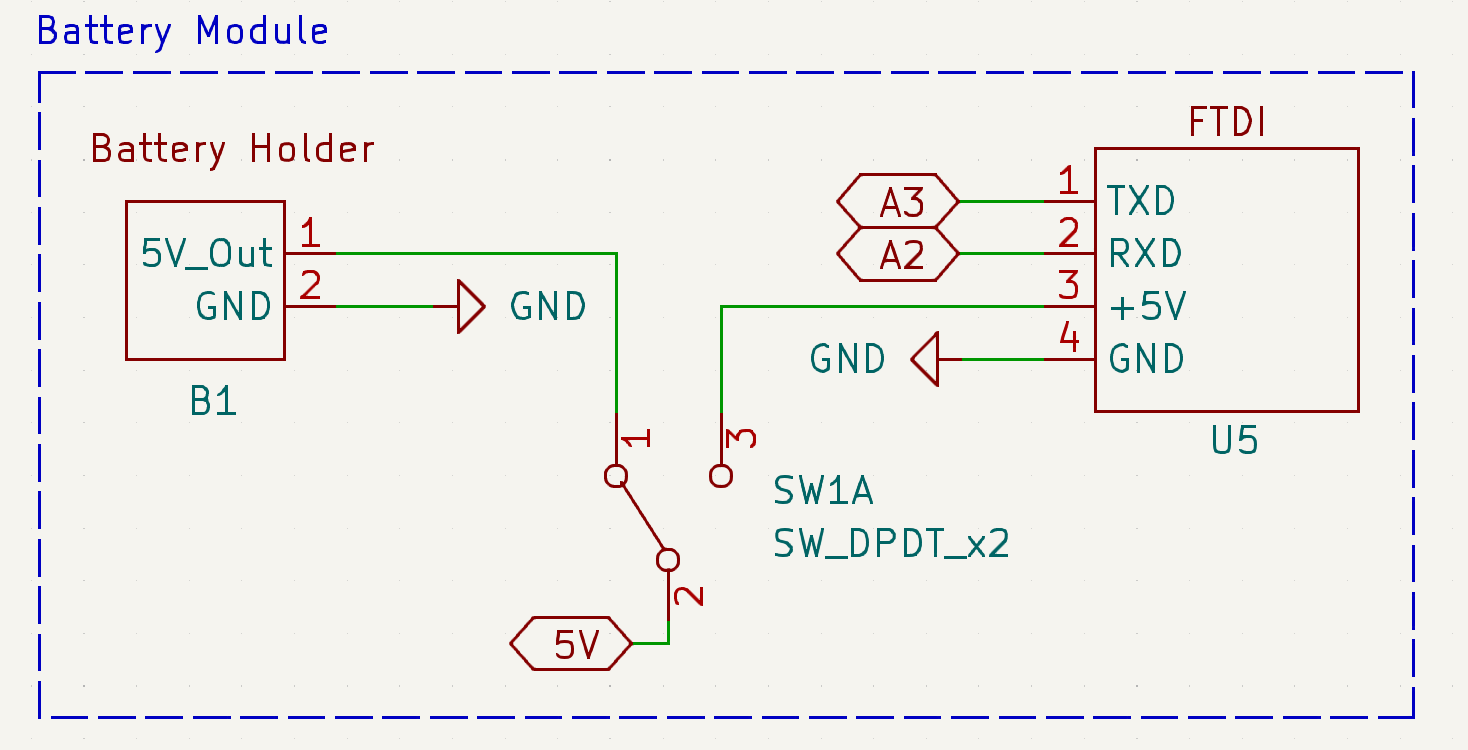
\includegraphics[width=0.6\linewidth]{../Images/batteryModuleSchematic.png}
    \caption{Battery Module Schematic}
    \label{fig:batterymoduleschematic}
\end{figure}

The battery module schematic contains the battery holder and charging circuit, as described in section \ref{sec:powercircuitry}, as well as the generic UART to USB adaptor. Additionally, I decided to add a switch to give the user of the transmission circuit the ability to change the power source for the circuit between the battery system itself, and the UART to USB adaptor. This switch adds a layer of safety to the circuit because it completely takes away the ability of the user to be able to feed power into the output of the battery module from the UART to USB convertor or to feed power into the USB of the computer from the output of the battery module. The switch implemented is a simple two-way toggle switch. Leading on from this, below in figure \ref{fig:sensormoduleschematic}, the schematic of the sensor module can be seen.


\begin{figure}[H]
    \centering
    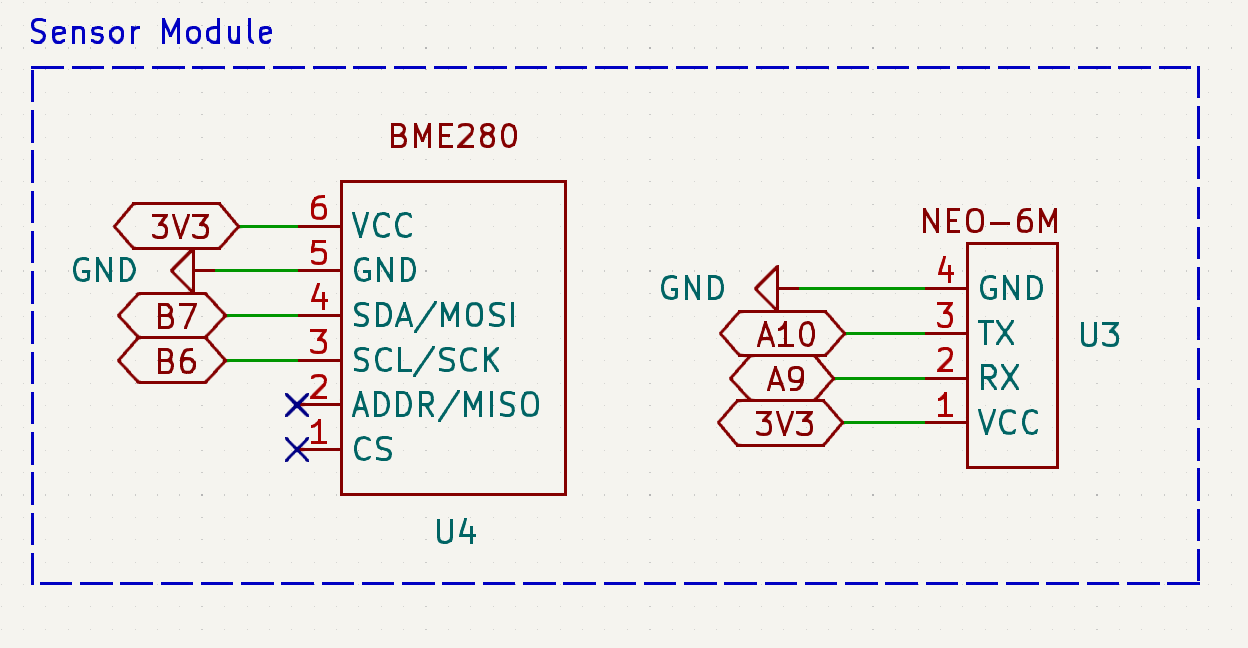
\includegraphics[width=0.6\linewidth]{../Images/sensorModuleSchematic.png}
    \caption{Sensor Module Schematic}
    \label{fig:sensormoduleschematic}
\end{figure}

The sensor module contains the BME280 for temperature, pressure and humidity measurements, and the NEO-6M for GPS measurements. As can be seen in the figure, the BME280 is connected to the microcontroller via the I2C pins and gets power from the 3.3V and GND rail coming from the microcontroller. The NEO-6M is also connected to the same power rails, however for communication, it is connected to a serial port on the microcontroller. In figure \ref{fig:loramoduleschematic} below, the LoRa module's schematic can be seen. As you can see, the LoRa module was connected to a 3.3V and GND power rail like the other sensors in the sensor module. The LoRa module is connected to the microcontroller via the SPI protocol. This connection can be seen via the NSS, MOSI, MISO, and SCK pins. The LoRa module also required a connection to the microcontroller from the reset pin and the DIO0 pin. The reset pin was to put the LoRa module in a reset state, and the DIO0 pin is a general-purpose pin that gives information about the LoRa transmission such as when the latest packet transmission has been completed.

\begin{figure}[H]
    \centering
    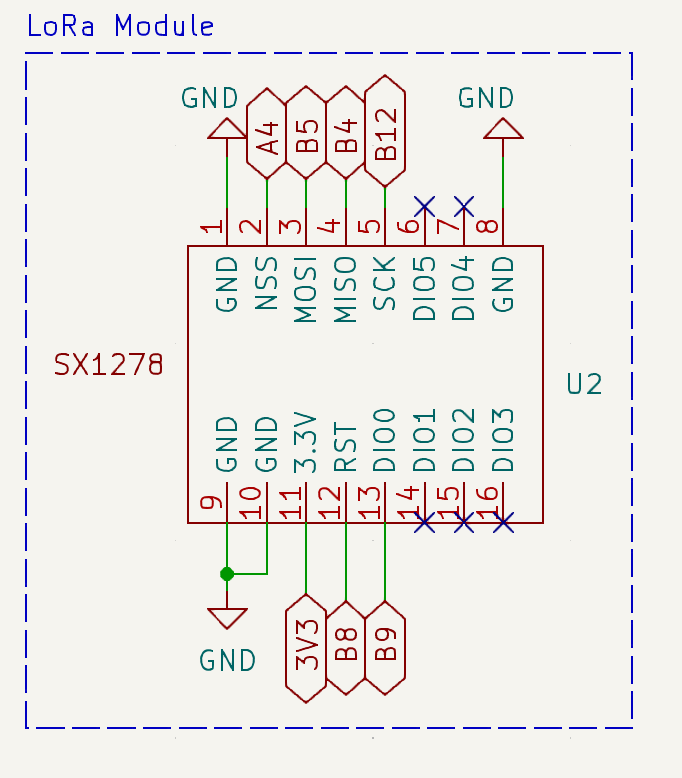
\includegraphics[width=0.55\linewidth]{../Images/loraModuleSchematic.png}
    \caption{LoRa Module Schematic}
    \label{fig:loramoduleschematic}
\end{figure}

Lastly, the schematic for the display and control module is shown below in figure \ref{fig:displayandcontrolmoduleschematic}. This module features the OLED display that is connected to the microcontroller via the I2C communication protocol and it also shows the two push button momentary switches which are going to be used for switching the parameters of the LoRa module on the transmission side. From the schematic, it can be seen that the push buttons connect specific GPIO pins, namely pins PB13 and PA5, to ground when they are pressed. The idea behind this was to minimise the physical components required to make the push buttons successfully interact with the microcontroller. By having buttons that simply connect certain GPIOs to ground, the design could employ internal pullup resisters that the STM32F411 has available to trigger an interrupt whenever a falling edge is detected at the specific GPIO pins connected to the push buttons. The exact workflow of this button input structure will be discussed in later sections.


\begin{figure}[H]
    \centering
    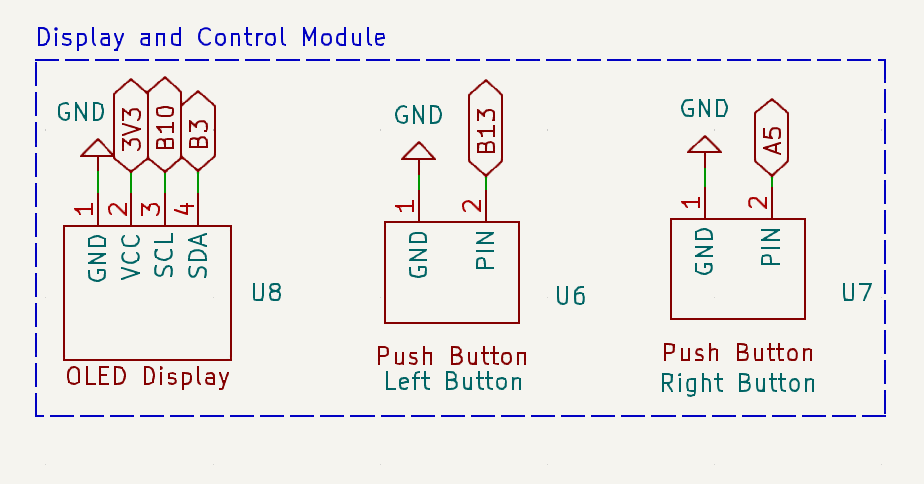
\includegraphics[width=0.6\linewidth]{../Images/displayAndControlModuleSchematic.png}
    \caption{Display and Control Module Schematic}
    \label{fig:displayandcontrolmoduleschematic}
\end{figure}

A full circuit schematic for the transmitter module can be found in appendix section \ref{appendix:fulltransmitterschematic}.


\subsection{Receive Module Interface Design}
The receive module is slightly simpler than the transmission module because it doesn't include any of the sensing devices, the external UART to USB convertor, or any battery circuitry. A rough overview of the circuit for the receive module can be seen in figure \ref{fig:receivemoduleinterfacing} below.

\begin{figure}[H]
    \centering
    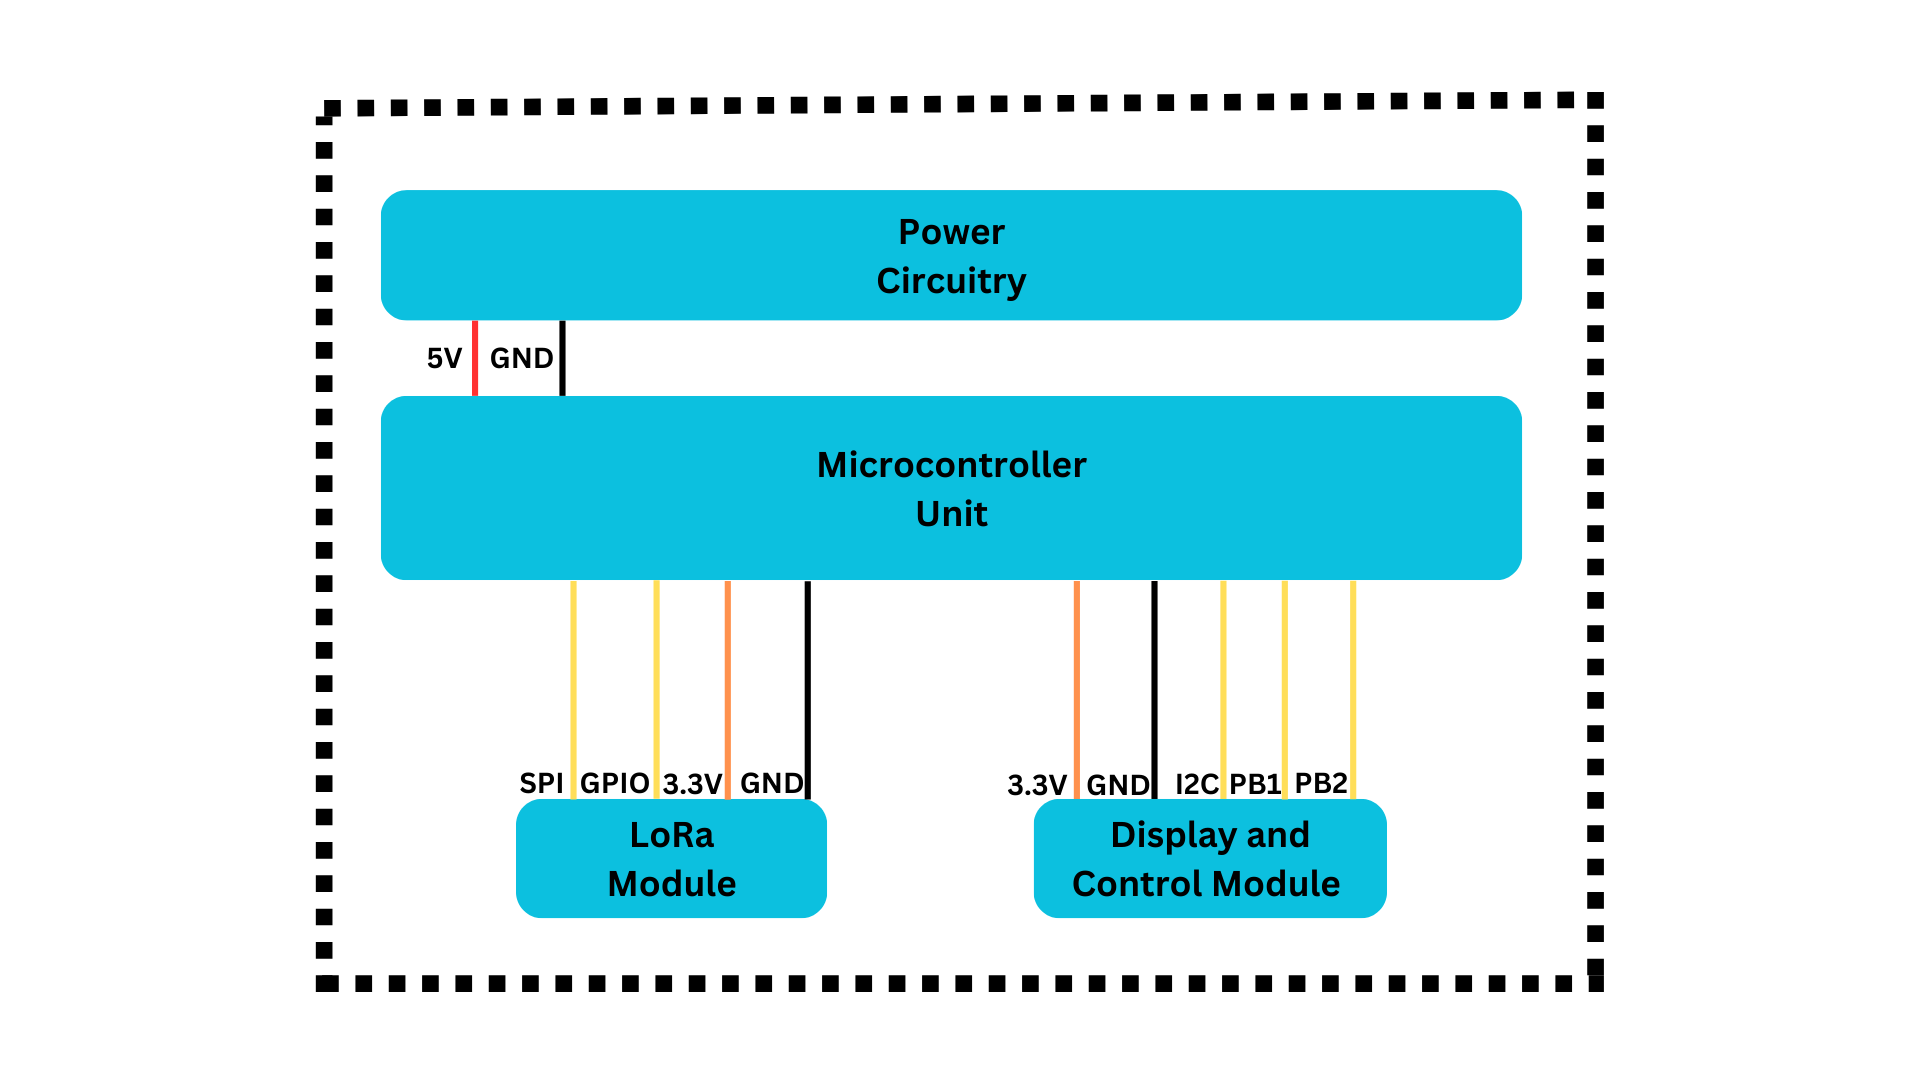
\includegraphics[width=0.8\linewidth]{../Images/receiveModuleInterface.png}
    \caption{Overview of the Interfacing with then Receive Module}
    \label{fig:receivemoduleinterfacing}
\end{figure}

It is clear from the above figure that there are far fewer components that make up the receive module. This is because the receive module doesn't need to have any sensors on it, and it doesn't need to be portable, meaning that a battery and charging module do not need to be implemented into the circuit. Figure \ref{fig:receivemodulemicrocontrollercircuit} below shows the circuit diagram for the receiver circuit's microcontroller module. 

\begin{figure}[H]
    \centering
    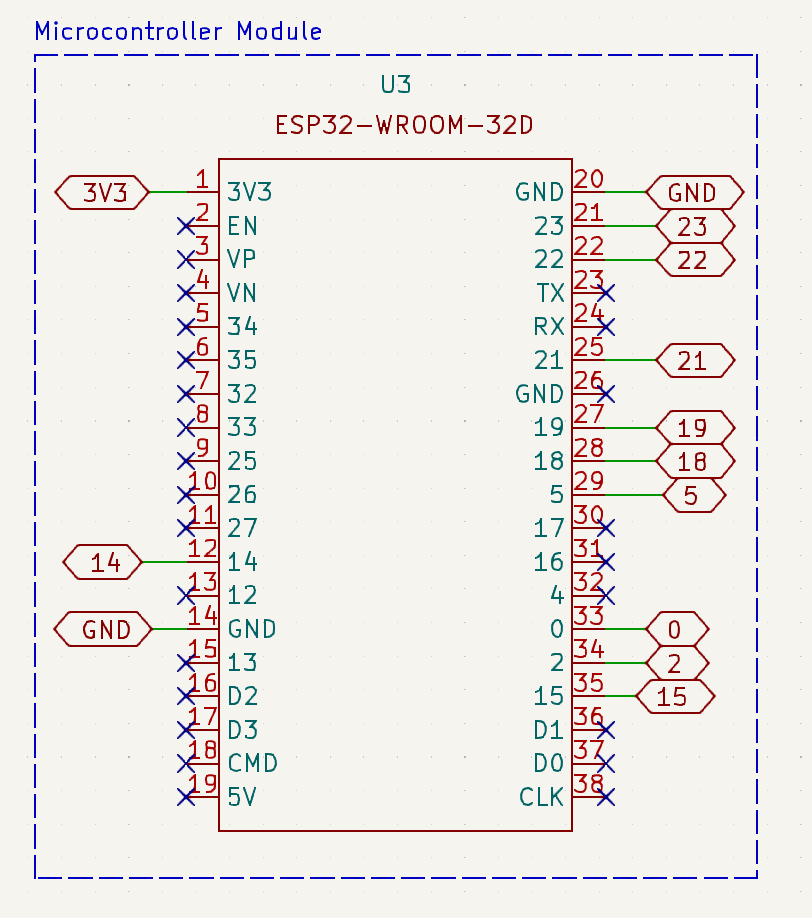
\includegraphics[width=0.5\linewidth]{../Images/receiverMicrocontrollerModuleSchematic.png}
    \caption{Receiver Module Microcontroller Circuit}
    \label{fig:receivemodulemicrocontrollercircuit}
\end{figure}

As you can see in the above image, the receiver circuit microcontroller doesn't have as many pins being utilised as the microcontroller for the transmitter circuit. This is due to the receiver circuit only implementing a microcontroller module, a LoRa module, and a display and control module. Much the same as the LoRa module for the transmission circuit, the LoRa module for the receiver circuit utilises the SPI communication protocol, with additional GPIO pins connected to RST and DIO0. This is shown below in figure \ref{fig:receivemoduleloracircuit} below.

\begin{figure}[H]
    \centering
    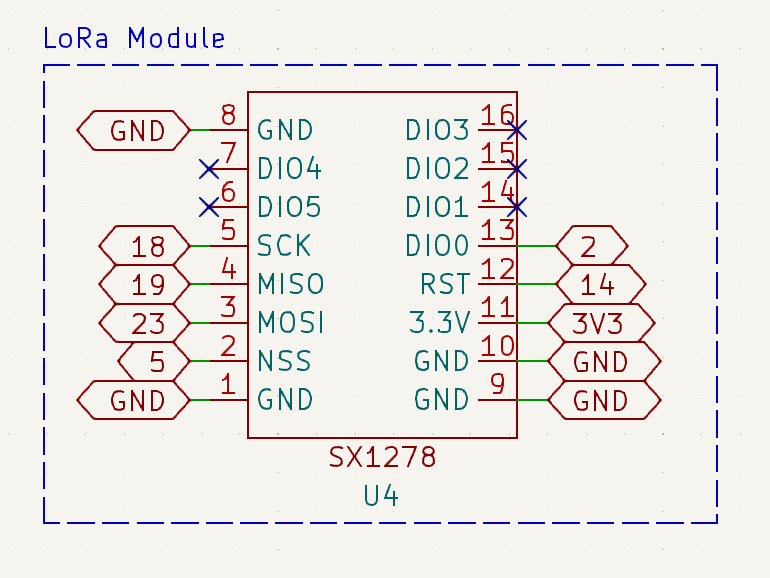
\includegraphics[width=0.6\linewidth]{../Images/receiverLoraModuleSchematic.png}
    \caption{Receiver Module LoRa Circuit}
    \label{fig:receivemoduleloracircuit}
\end{figure}

Lastly, much like the transmitter circuit, the receiver circuit needs a display and control module. This circuit is shown below in figure \ref{fig:receivemoduledisplayandcontrolcircuit}. This circuit is exactly the same as the display and control circuit for the transmitter module and features the same design of the push buttons connecting to specific GPIO pins, in this case, pins 15 and 0 for the left and right buttons respectively, which use pull up resisters and interrupts to trigger certain functions into action when their respective GPIO pins are connected to ground.

\begin{figure}[H]
    \centering
    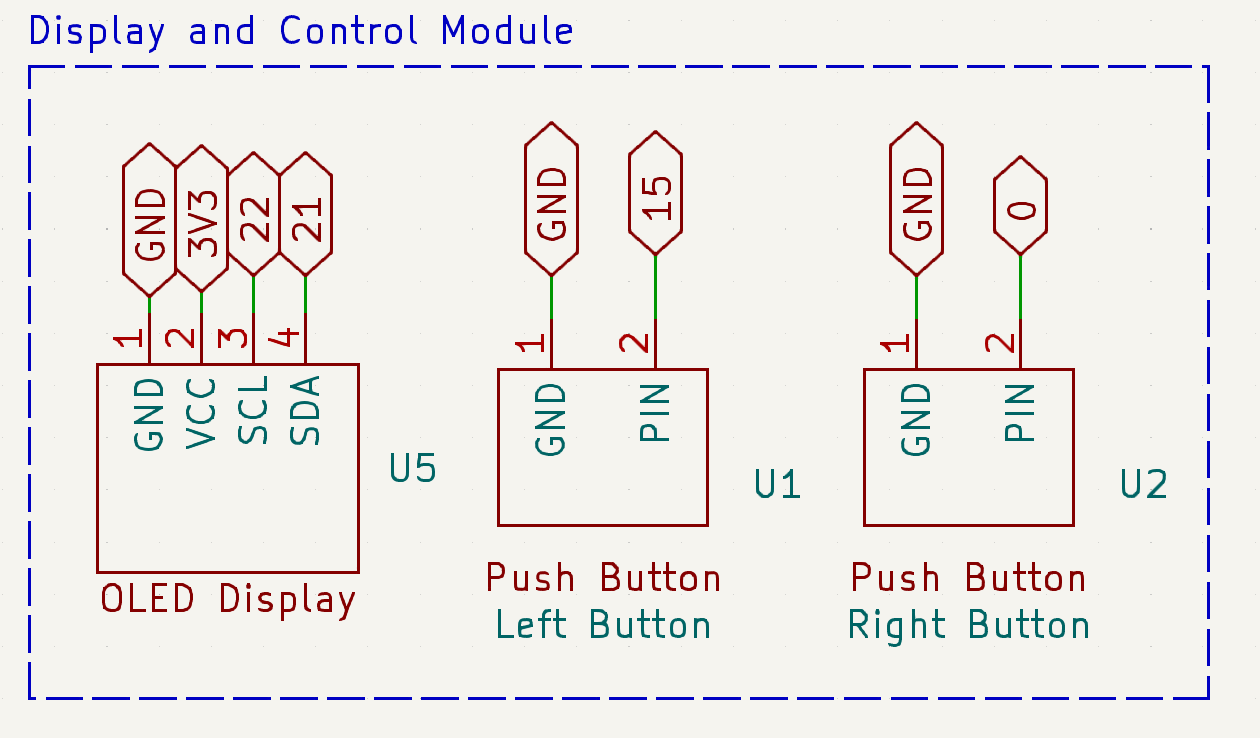
\includegraphics[width=0.6\linewidth]{../Images/receiverDisplayAndControlModuleSchematic.png}
    \caption{Receiver Module Display and Control Circuit}
    \label{fig:receivemoduledisplayandcontrolcircuit}
\end{figure}

A full schematic of the receiver module can be found in section \ref{appendix:fullreceiverschematic} of the appendix.

\subsection{Implementation of Transmission Circuit Design}
The design of the transmission circuit was implemented on 2.54mm stripboard. This stripboard is perfect for prototypes because as mentioned before, they allow for a less noisy design environment than breadboards. In figure \ref{fig:stripboardimplementationoftransmissioncircuit} below, the transmission circuit prototype is pictured. The front and back side of the stripboard is shown. The stripboard design included the use of female pin headers for all the components in the circuit. This was done to ensure that the components could be easily removed from the prototype to make testing and building the circuit easier. Doing the prototyping this way also gave me the ability to potentially remove components for placement on a PCB that was designed. All the components were hand-soldered onto the stripboard over the course of a few days.

\begin{figure}[H]
    \centering
    \begin{subfigure}{0.45\textwidth}
        \centering
        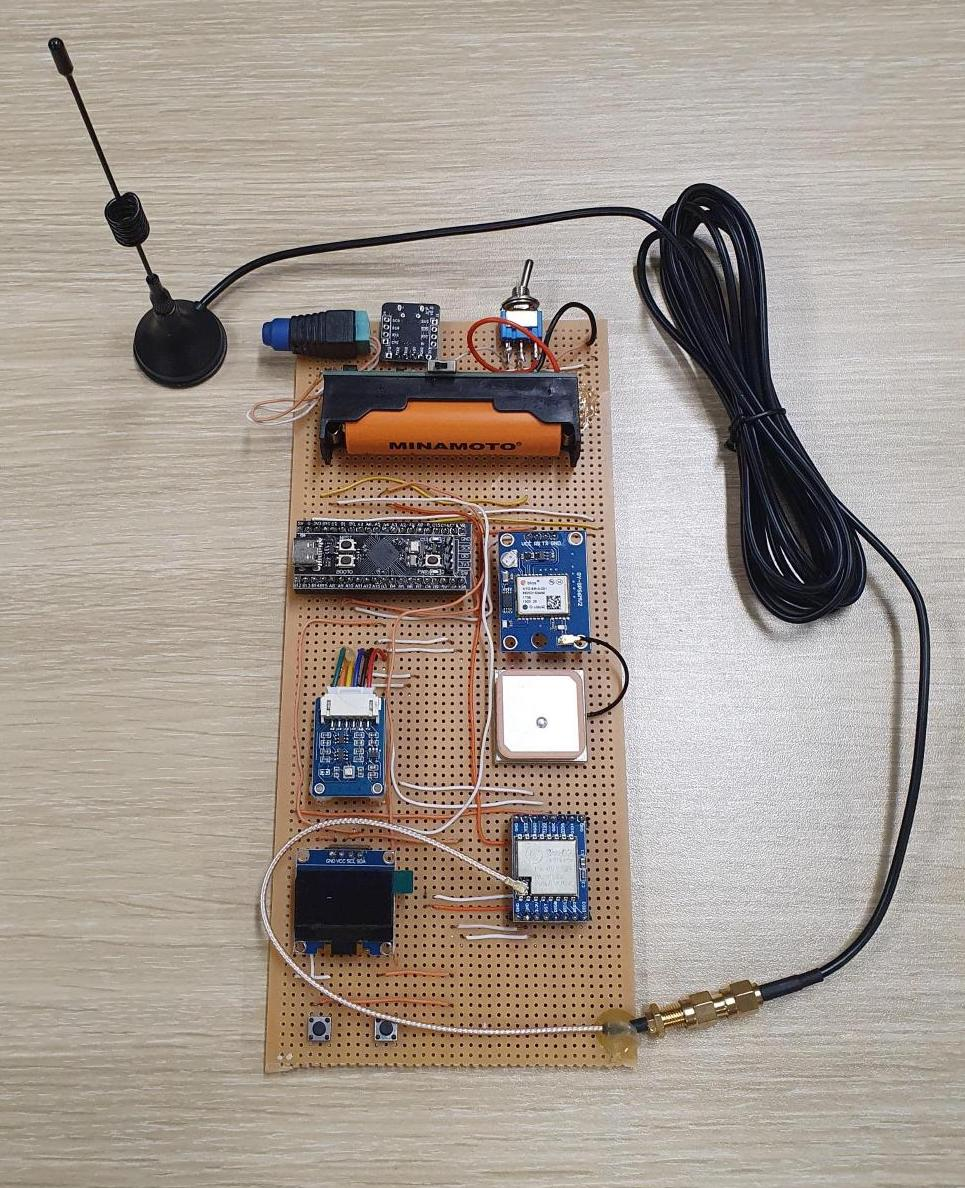
\includegraphics[width=\textwidth]{../Images/transmissionCircuitStripboardFront.jpeg}
        \caption{Implementation of Transmission Circuit on Stripboard Front}
    \end{subfigure}\hfill
    \begin{subfigure}{0.45\textwidth}
        \centering
        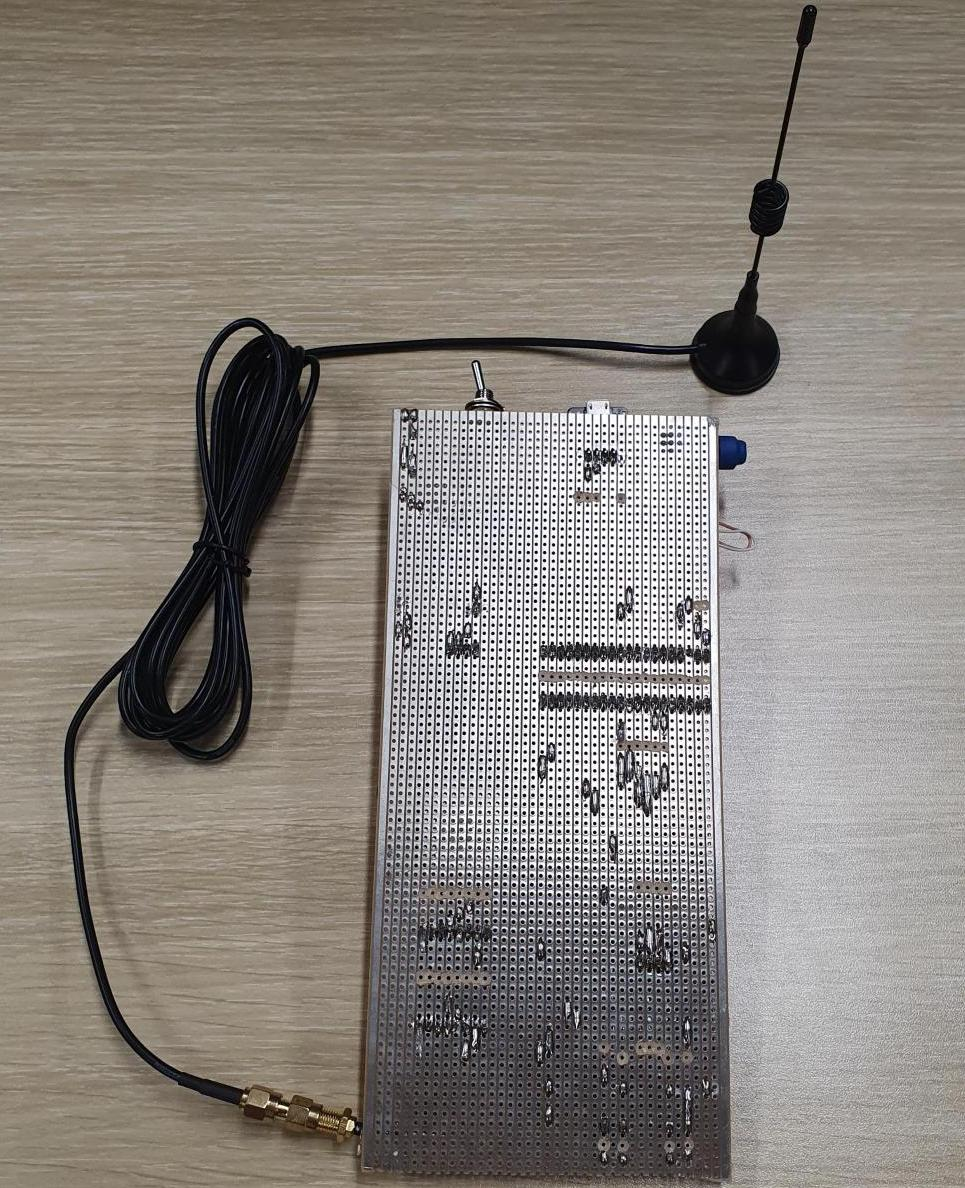
\includegraphics[width=\textwidth]{../Images/transmisionCircuitStripboardBack.jpeg}
        \caption{Implementation of Transmission Circuit on Stripboard Back}
    \end{subfigure}
    \caption{Stripboard Prototype of Transmission Circuit}
    \label{fig:stripboardimplementationoftransmissioncircuit}
\end{figure}


\subsection{Implementation of Receiver Circuit Design}
Much like the transmission circuit outlined above, the receiver circuit was also built on 2.54mm stripboard since it provides such a good platform to prototype with. Similar to the transmission circuit, female pin headers were utilised in the creation of the receiver circuit, this allowed for some flexibility in prototyping, especially considering the fact that I wanted to manufacture a PCB for the transmission and receiver circuits eventually, which would require removing certain components from the prototype board. The physical implementation of the receiver circuit design can be seen in figure \ref{fig:stripboardprototypeofreceivercircuit} below.

\begin{figure}[H]
    \centering
    \begin{subfigure}{0.45\textwidth}
        \centering
        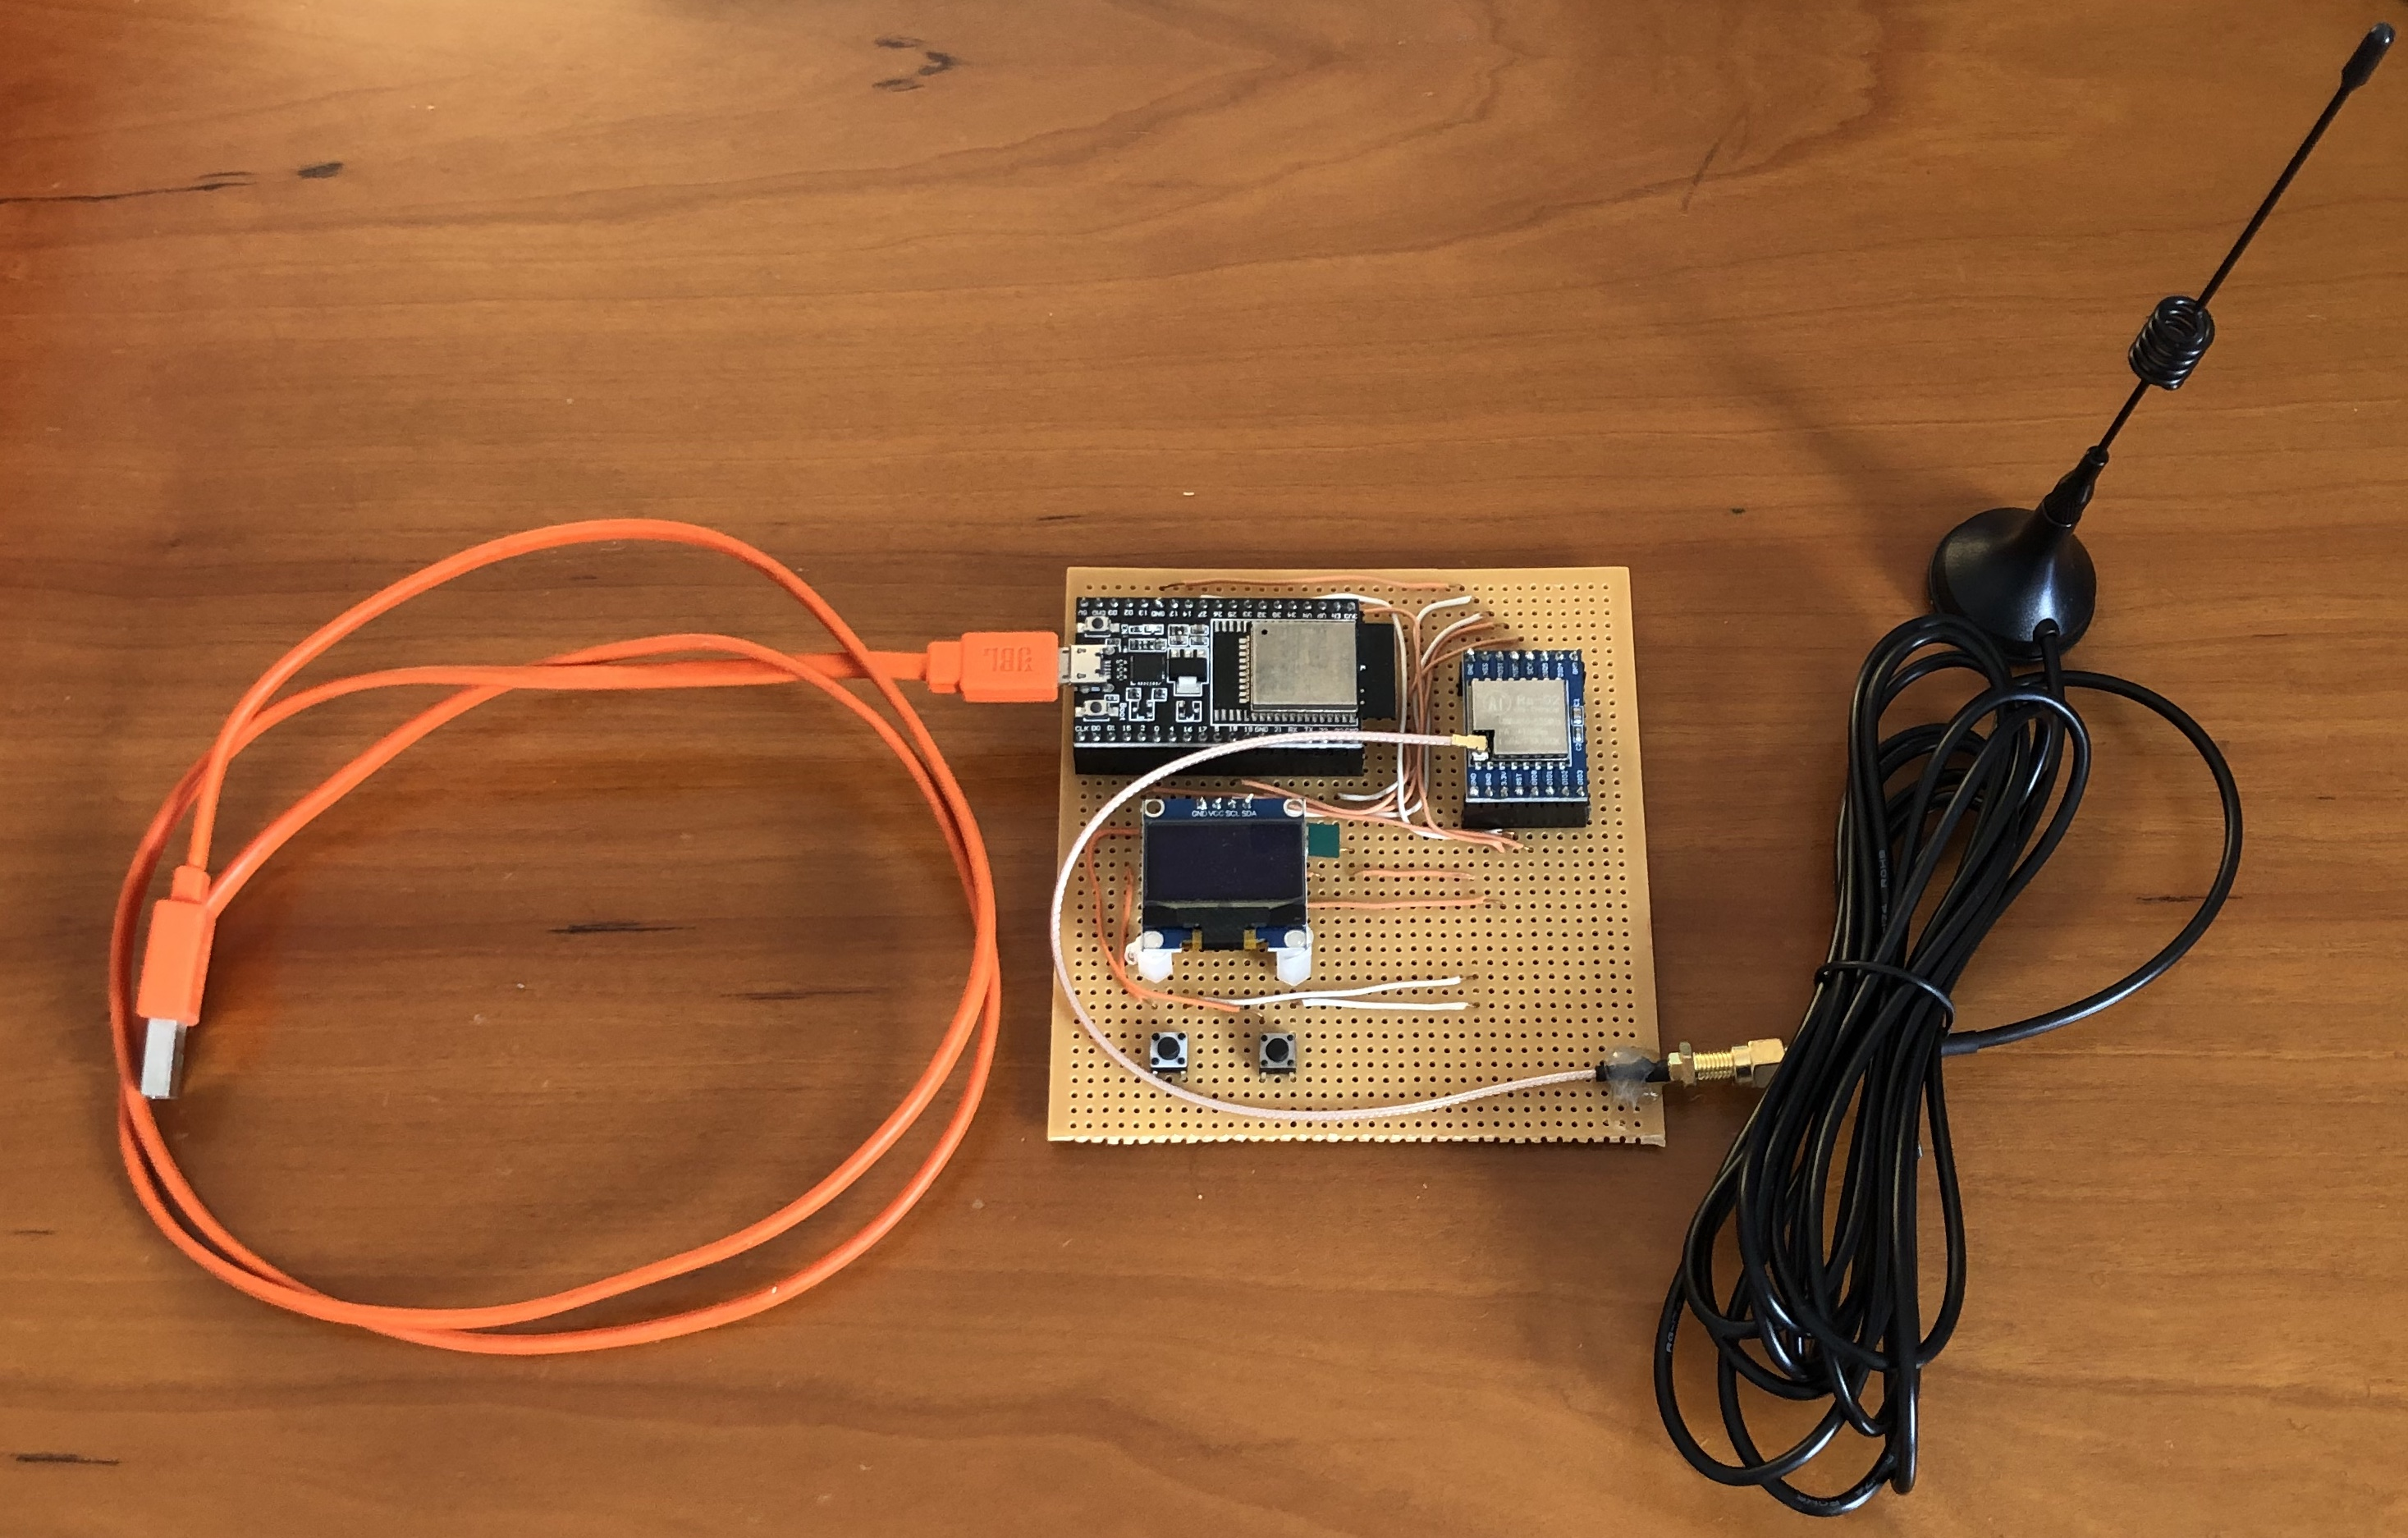
\includegraphics[width=\textwidth]{../Images/receiverFrontSide.jpg}
        \caption{Implementation of Receiver Circuit on Stripboard Front}
    \end{subfigure}\hfill
    \begin{subfigure}{0.45\textwidth}
        \centering
        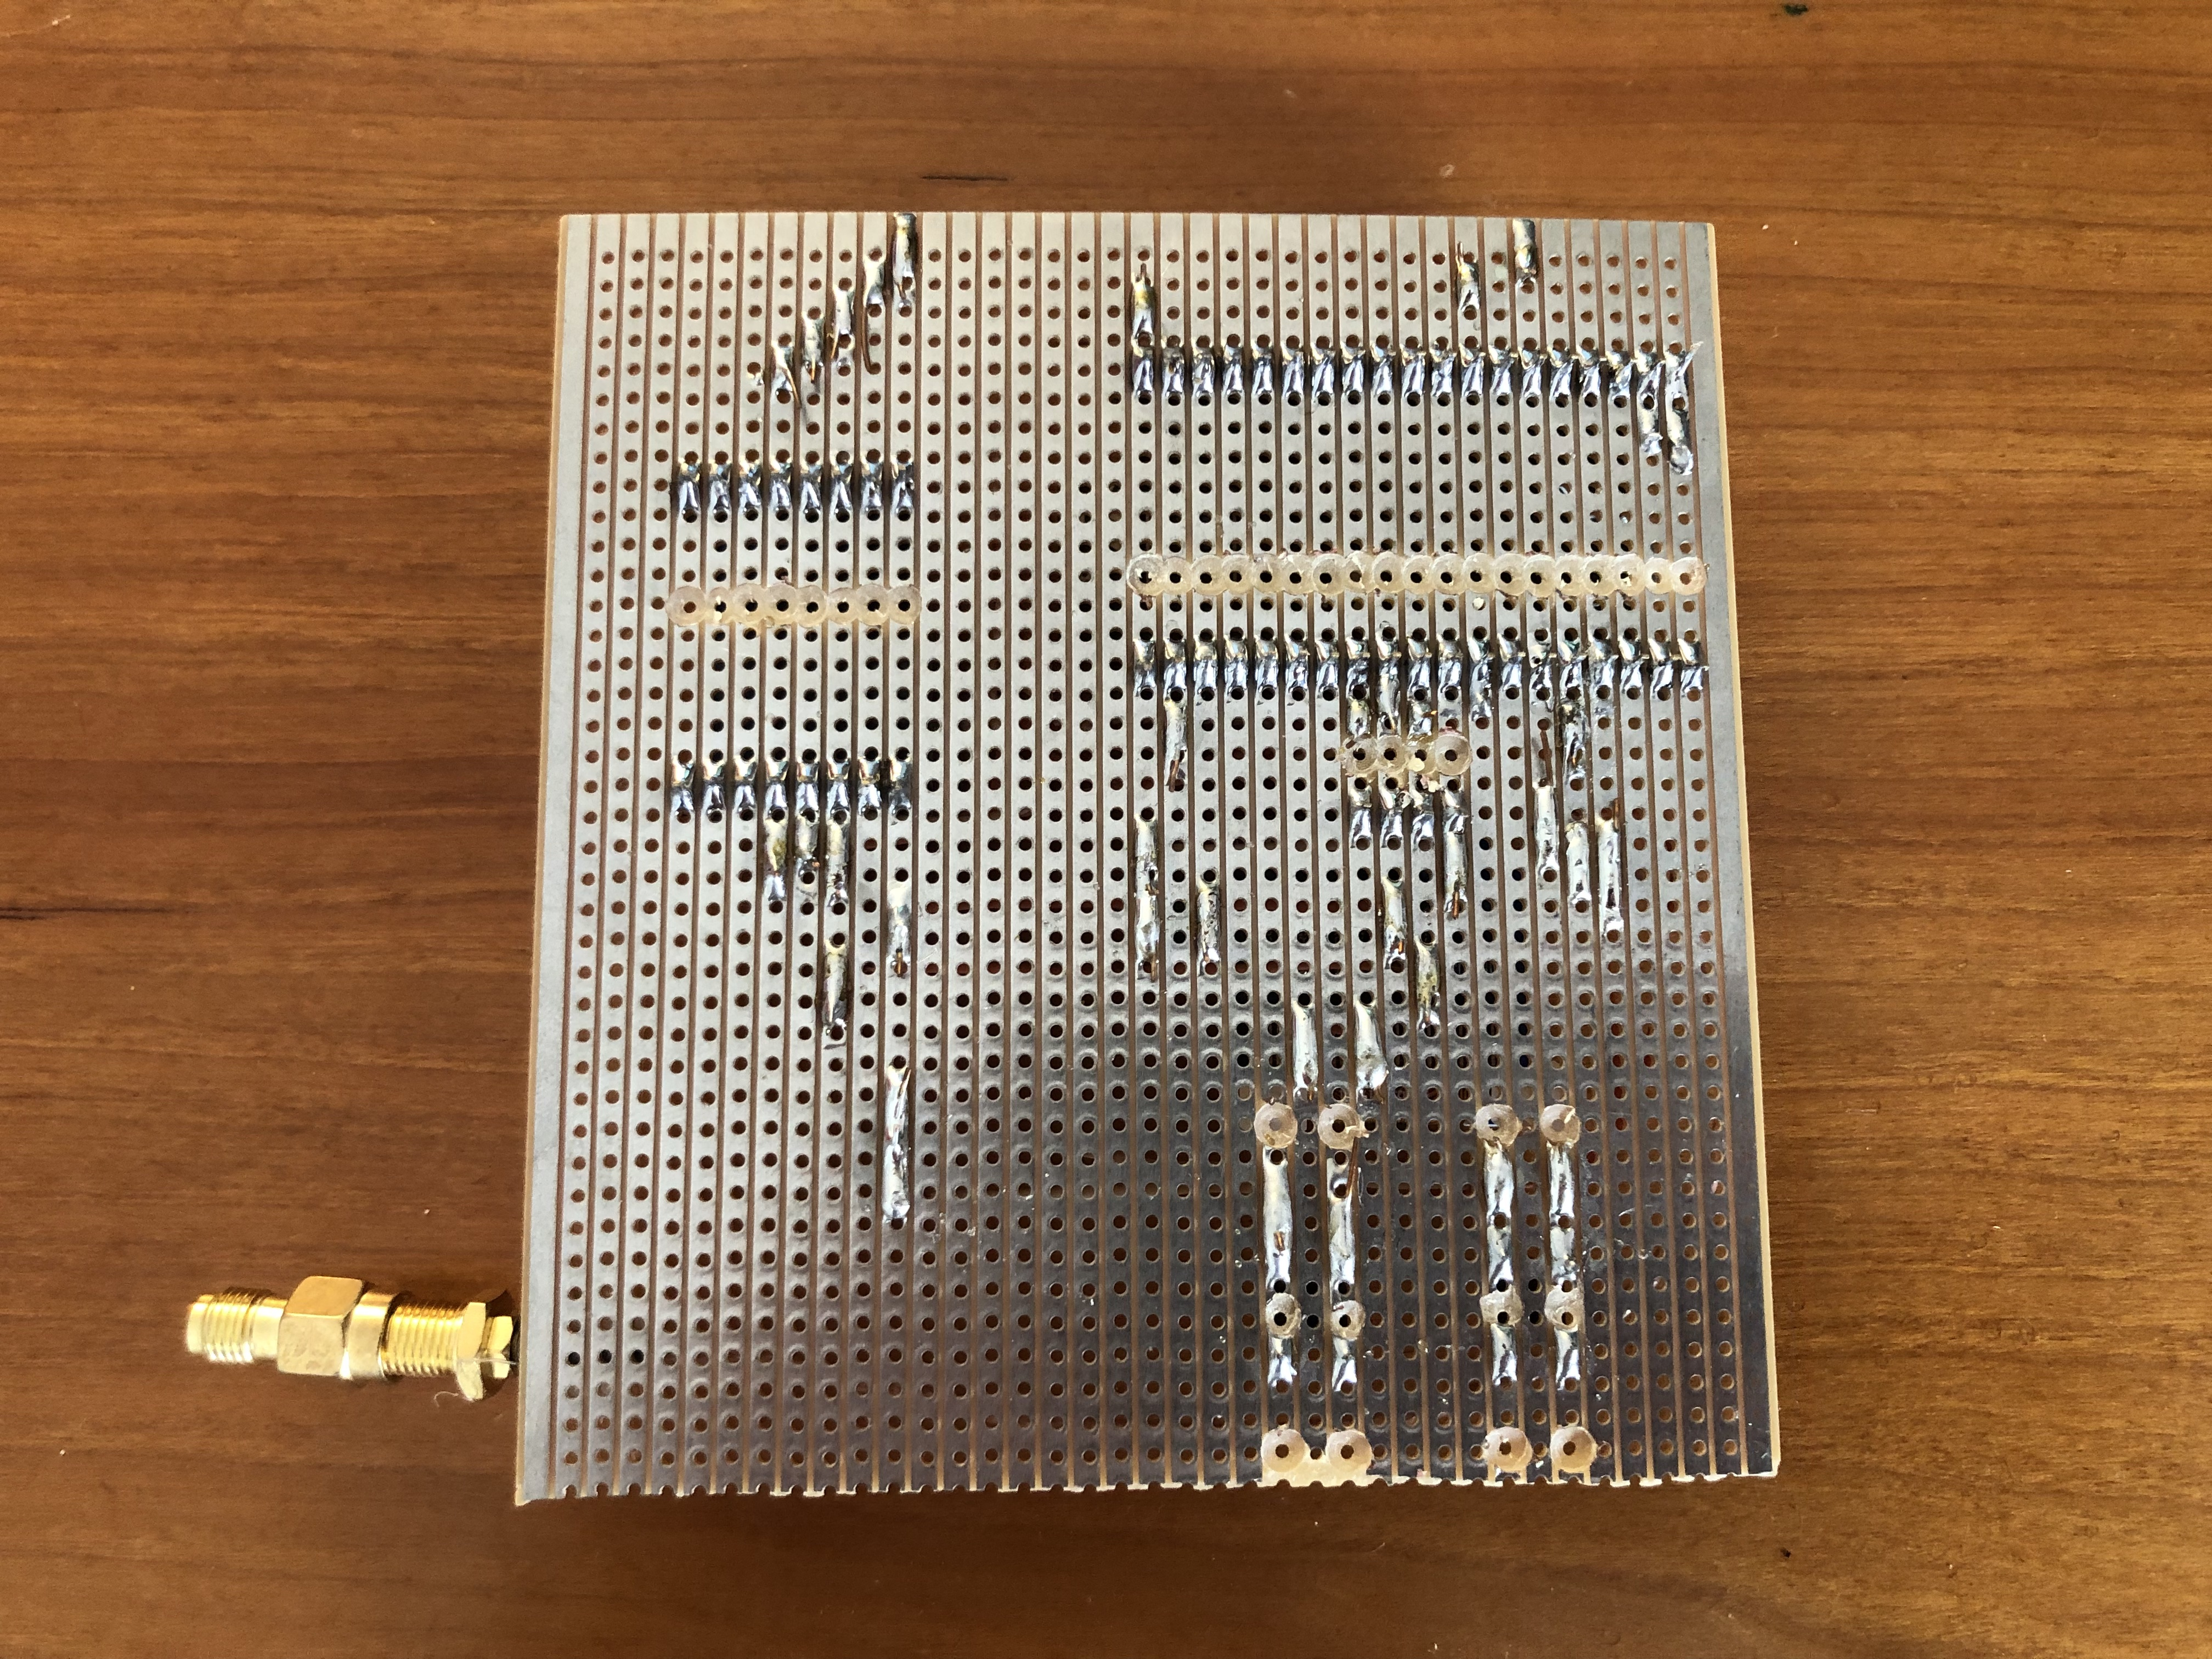
\includegraphics[width=\textwidth]{../Images/receiverBackSide.jpg}
        \caption{Implementation of Receiver Circuit on Stripboard Back}
    \end{subfigure}
    \caption{Stripboard Prototype of Receiver Circuit}
    \label{fig:stripboardprototypeofreceivercircuit}
\end{figure}


\section{Software Design}\label{sec:softwaredesign}
The software design for both the transmitter circuit and the receiver circuit came with many challenges along the way, however, a lot of valuable information was learnt from the process that can be taken forward. The following sections outline the software design thinking process and steps taken in the design of the software itself. It must be noted, that any code snippets shown in the following sections are merely rough representations of specific parts of the overall software and are in place to show the rough working of specific parts of the overall software. The main code in its entirety for either the transmitter or receiver circuits can be found at the following GitHub link: \href{https://github.com/roryschram/EEE4022S_Final_Project}{https://github.com/roryschram/EEE4022S\_Final\_Project} as seen in appendix section \ref{appendix:githublink}.

\subsection{Software Design and Implementation for Transmission Circuit}
Since the transmitter circuit was based around the STM32F411 microcontroller, it was decided that the best tech stack to use was the following.
\begin{enumerate}
    \item \textbf{STM32CubeMX}: This software plays a big role in the initial setup of the STM32F411 device itself. It helps to create all the required boilerplate code for the STM32 for things such as communication interface setup, timer setup, clock setup, and GPIO setup. This piece of software plays a crucial role in the development process for the STM32F411 since it eases the design process of the software quite dramatically.
    \item \textbf{VSCode}: VSCode was used as the text editor of choice due to its large extension library and my personal experience with the software over the past four years allowing me to have a firm understanding of its capabilities.
\end{enumerate}

With these three pieces of software, the flashing and debugging of the STM32 became an easy process. As mentioned previously, the STM32F411 does not have a built-in debugger, and therefore an external debugger had to be used. In my case, the easiest debugger to use that I had on hand was the built-in debugger within the STM32F0 Discovery Development Board. It was a simple process of disconnecting some pins on the STM32F0 Discovery Board to enable the debugger to be used on an external device such as the STM32F411. The hardware debugging process can be seen in figure \ref{fig:debuggercircuit} below.

\begin{figure}[H]
    \centering
    \begin{subfigure}{0.45\textwidth}
        \centering
        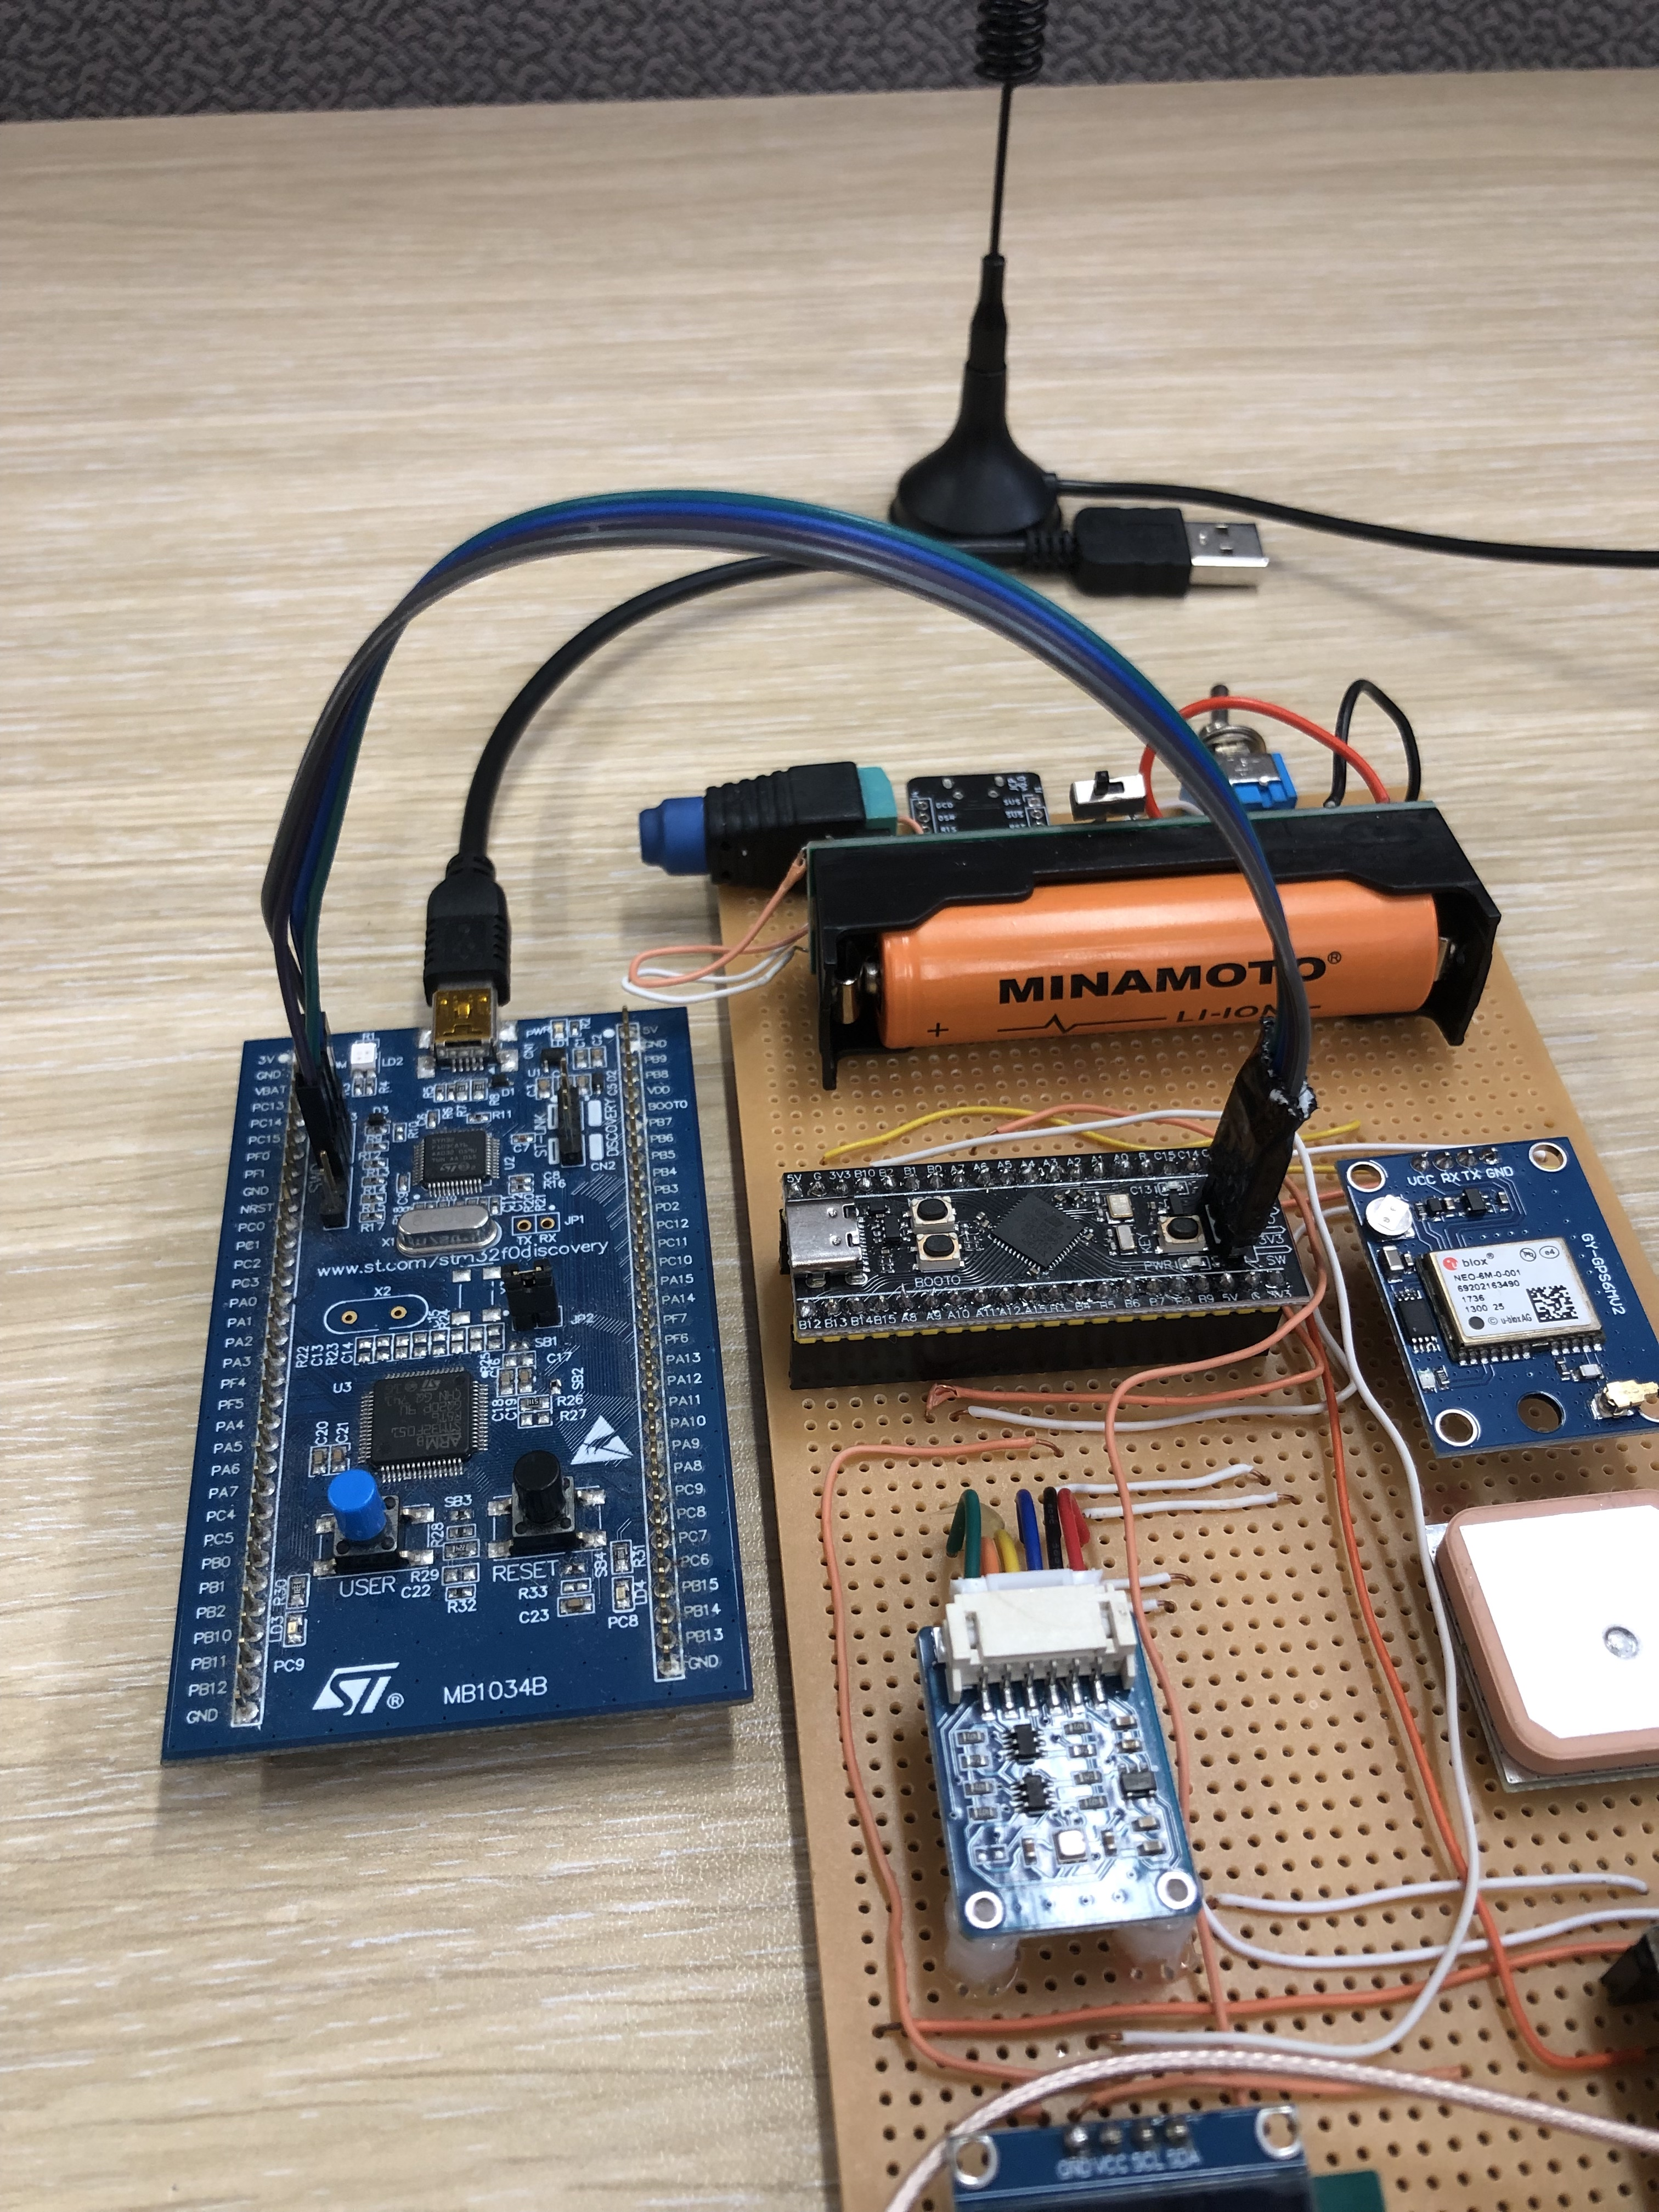
\includegraphics[width=\textwidth]{../Images/debuggerCircuitPicture1.jpg}
        \caption{Ribbon cable between debugger and microcontroller}
    \end{subfigure}\hfill
    \begin{subfigure}{0.45\textwidth}
        \centering
        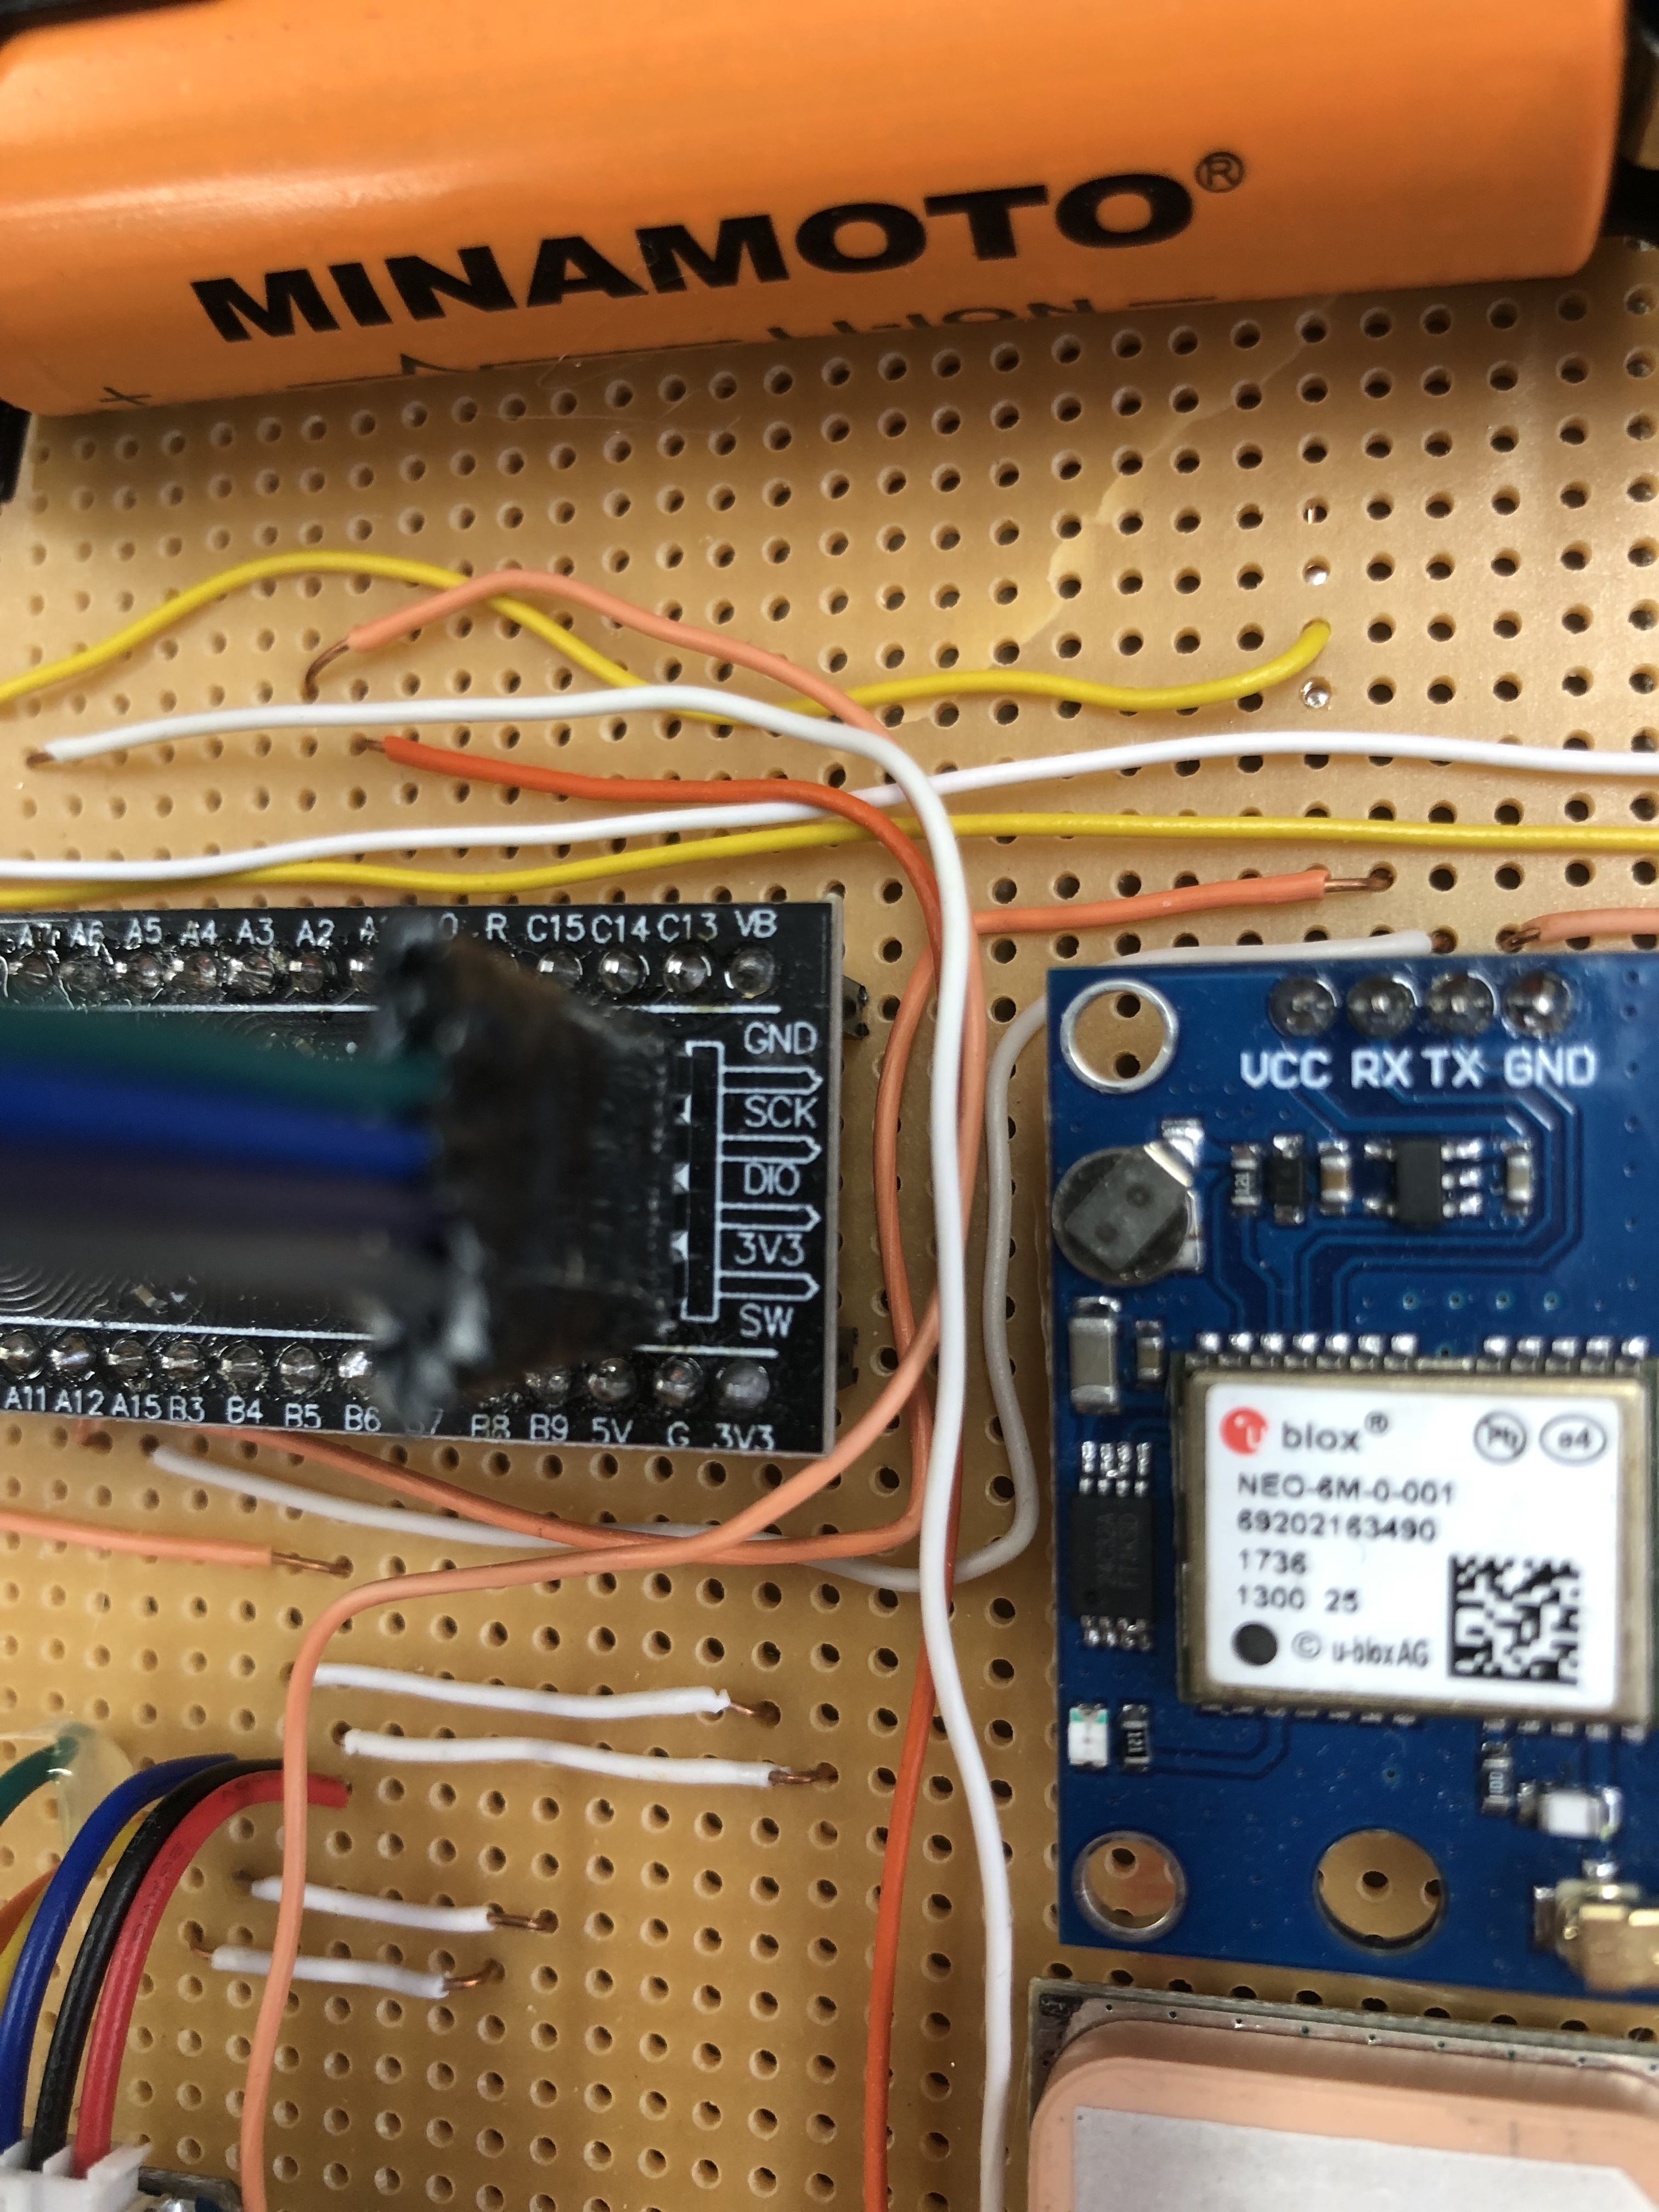
\includegraphics[width=\textwidth]{../Images/debuggerCircuitPicture2.jpg}
        \caption{Close up of connection between microcontroller and debugger}
    \end{subfigure}
    \caption{Debugger Circuit}
    \label{fig:debuggercircuit}
\end{figure}

The next task that had to be completed, was to design a rough workflow of how the software would handle the reading and processing of the data in the transmission module. In figure \ref{fig:transmissioncircuitsoftwareflowchart} below, the final flow chart for the transmitter can be seen. This flow chart was only finalised after many iterations of the software were completed. For me personally, designing software using the iterative design approach is more beneficial than designing a final prototype from the get-go. This is because designing with an iterative approach gives the designer more flexibility and adaptability to slightly changing requirements along the path of the design process. This gave me the ability to adapt to certain challenges which popped up during the prototyping stage of development.
\begin{figure}[H]
    \centering
    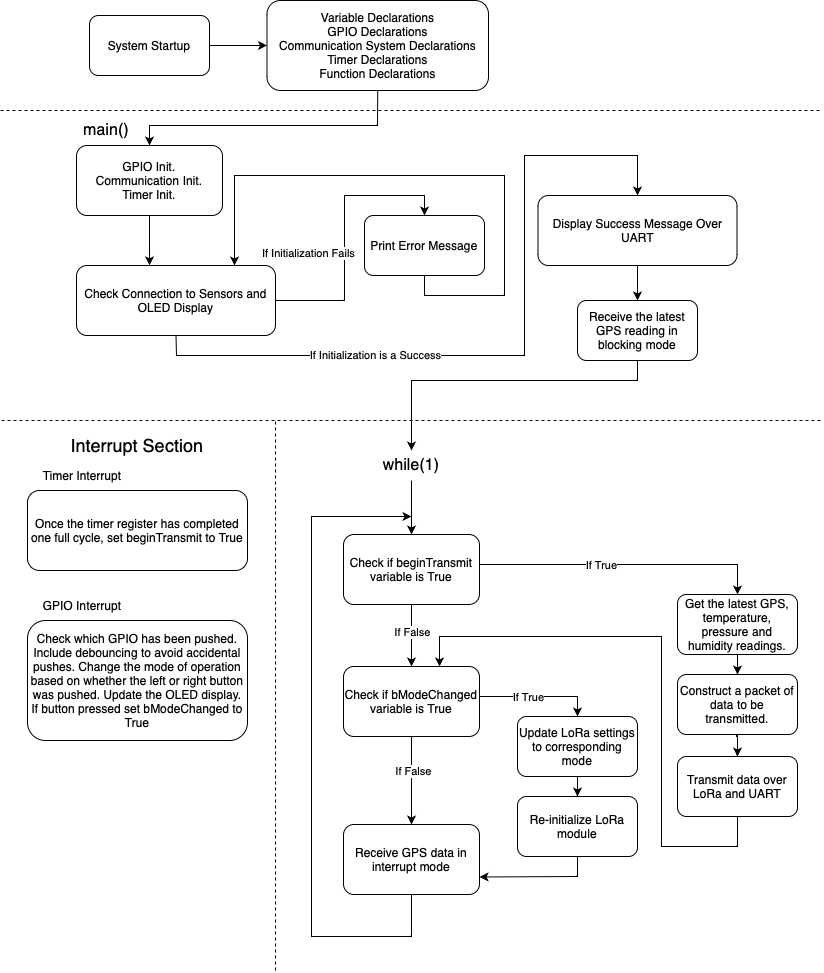
\includegraphics[width=0.7\linewidth]{../Images/transmissionCircuitSoftwareFlowChart.png}
    \caption{Flow Chart of the Transmission Circuit Software}
    \label{fig:transmissioncircuitsoftwareflowchart}
\end{figure}

To give a brief overview of the final flowchart shown above, it all starts when the system is powered up. At power-up, the various global variables that are used in the software are initialised, as well as the data structures that the STM32CubeMX software produces for the GPIOs, the communication systems, and the timers. The functions contained within the software are also defined here. 

After this, the main() function begins. In this function, all the various necessary initialisation takes place, such as the initialisation for the GPIOs, the communication systems, the timers, the sensors, and the OLED display. If the initialisation for the sensors fails, then an error message is printed and the program keeps trying to initialise the sensors. If the initialisation is successful, then a success message is printed over UART. After this, a packet of raw GPS data is received in blocking mode so that the system has data to transmit from the get-go if a timer interrupt is immediately called.

The next thing that happens is the main while loop begins. The first thing that this while loop does is check if the beginTransmit boolean is set to true. This boolean gets set to true via a timer interrupt outlined in the interrupt section of figure \ref{fig:transmissioncircuitsoftwareflowchart}. Essentially, once the timer register rolls over, then an interrupt is called and in that interrupt function, the beginTransmit boolean is set to true. This boolean dictates when a packet of LoRa data must be transmitted. How often it triggers is dependent on the value set in the \gls{arr} for that specific timer. The way in which the ARR was setup for this experimental design allowed for intervals ranging from 1 - 60 seconds between LoRa transmissions. If beginTransmit is true, then the latest GPS data is read, as well as the latest temperature, pressure and humidity values.

\subsubsection{Reading GPS Data}
The NEO-6M GPS module was the first of the sensors which I started developing software for. The default parameters for the NEO-6M are to send a \gls{gps} \gls{nmea} packet over serial at a frequency of 1Hz. The GPS NMEA packet structure is a standardised communication data structure for raw GPS data \cite{GPS_NMEA_DATA}. To do this, I settled on using the HAL's built-in function called HAL\_UARTEx\_ReceiveToIdle\_IT(). This function receives a serial communication until a certain number of bytes have been received, or until the serial communication goes idle. An idle event in this case would be the end of a transmission of raw GPS data from the NEO-6M module. So essentially this function will receive data from the NEO-6M until the data stops sending, and it will store this raw data in a memory location of our choosing. To parse the NMEA data, I used the popular open source library called "minmea"\footnote{The minmea library can be found \href{https://github.com/kosma/minmea}{here}.}. The HAL\_UARTEx\_ReceiveToIdle\_IT() function is a non-blocking function. Using a non-blocking function to read the GPS data was important because it allowed the GPS data to be read in the background. This was necessary because the GPS data was sent from the GPS module every 1 second, and if a blocking function was used to read the data, then it could cause timing issues.

\subsubsection{Reading Temperature, Pressure, and Humidity Data}
The reading of the temperature, pressure, and humidity values was a much more streamlined and simple process than the GPS data. I utilised an opensource library written specifically for the BME280\footnote{The BME280 library can be found \href{https://github.com/ciastkolog/BMP280_STM32}{here}.}. This library took care of the communication between the STM32F411 and the BME280 sensor. This communication was, as previously mentioned, achieved over I2C. The various values were read from the BME280 and then saved to individual variables. The altitude could be calculated from the pressure data.

\subsubsection{Calculating Altitude}
The rough altitude of the module can be calculated using one of the barometric equations that dictate the relationship between air pressure and altitude. This is shown below in equation \ref{eq:barometricformula}:
\begin{equation}
    h=h_{b}+\frac{T_{b}}{L_{b}}\left[\left(\frac{P}{P_{b}}\right)^{\frac{-RL_{b}}{g_{0}M}}-1\right] \label{eq:barometricformula}
\end{equation}

where
\begin{itemize}
    \item $h_{b}$ is the starting altitude that you want to measure from. In this case, the measurement is being taken from sea level, therefore $h_{b}$ is 0m.
    \item $T_{b}$ is the standard temperature at sea level in Kelvin. the standard value for this is 15\textdegree C, which is 288.15 K.
    \item $L_{b}$ is the standard temperature lapse rate in K/m. The standard for this value is -0.0065 K/m.
    \item $P$ is the current pressure in Pa.
    \item $P_{b}$ is the pressure at sea level in Pa. The standard value for this is 101325 Pa.
    \item $R$ is the universal gas constant, which for air is 8.31432.
    \item $g_{0}$ is the earth's gravitational acceleration constant, which is 9.80665.
    \item $M$ is the molar mass of air, which is 0.0289644 kg/mol.
    \item $h$ is the height measured in metres.
\end{itemize}

\subsubsection{Construction of Data Packet}\label{sec:contructionofdatapacket}
Once all the sensor data has been read from the various sensors, the next step was to construct a data packet. A data packet consisted of the following format defined by me. 

\lstset{
    literate={\\\%}{\%}1, % Replace \% with %
}
\begin{lstlisting}[caption={Full Data Packet Format}, label={lst:datapacketformat}]
Time(UTC + 0)|(Latitude(ddmm.mmmm),Longitude(ddmm.mmmm))|Pressure(Pa)|Temperature(C)|Humidity(\%)|Altitude(m)
\end{lstlisting}

First in the packet goes the time gathered from the GPS module, which is UTC + 00:00. The time is in the format of hh:mm:ss. Next, we deal with the GPS coordinates, first the latitude and then the longitude. Both the latitude and longitude are in the format of ddmm.mmmm as opposed to the more common dd.dddd format used today. The conversion to dd.dddd, or decimal degrees and fractions of a decimal degree, can be done by taking the dd portion of the latitude or longitude, and then concatenating on the mm.mmmm portion divided by 60. For example, these latitude and longitude co-ordinates, (-335745567,182936229), are given in the ddmm.mmmmm format and can be converted as follows. First, the whole number part of the latitude in the dd.dddd format will be -33 with the decimal part being the decimal part of the calculation of the mm.mmmmm part divided by 60. This decimal part is 57.45567/60=0.9575945. Therefore the final latitude is -33.9575945. Applying the same process to the longitude gives that the longitude in dd.dddd format is 18.4893715. The final coordinates are therefore (-33.9575945,18.4893715). The next step was to transmit the data over LoRa.

\subsubsection{Transmitting Data}
Once the packet of data was built, it could then be transmitted. To do this, a proper interface had to be established between the STM32F411 and the SX1278 LoRa module. This was done with the help of an open-source library designed for the STM32 architecture\footnote{The LoRa library can be found \href{https://github.com/SMotlaq/LoRa}{here}.}. This library gave the ability to simply transmit a string (or in the case of C, a char array), with one function call. As can be seen in figure \ref{fig:transmissioncircuitsoftwareflowchart} above, once the data was transmitted, the program then checks if bModeChanged variable is true. This is the check that happens to determine whether or not the mode of the board has been changed.

\subsubsection{Handling Mode Changes}
The board modes can be changed by pushing one of two push buttons located at the bottom of the transmitter circuit. These buttons can be seen at the bottom left of the transmitter module in figure \ref{fig:stripboardimplementationoftransmissioncircuit}. When either of these buttons are pushed, they simply ground the GPIO pins to which they are connected. The GPIOs that they are connected to are in pull-up resister mode. This means that they are nominally pulled high, and when the buttons are pressed, they cause a falling edge that can be detected by the GPIOs and an interrupt can be called. The reason for using this method of button detection was that it minimised the number of components needed to implement a button. In fact, the only component needed was the button itself, no other external circuitry. Once an interrupt was called, button debouncing was implemented in the software. This debouncing just made sure that there was adequate time between button pushes so as to avoid the micro-pushes caused when the momentary buttons are activated. After debouncing, a global mode variable is updated to correspond to an increase or decrease in the mode, depending on what button was pushed, the OLED display is updated with the current mode, and the bModeChanged boolean is set to true. That bModeChanged boolean is the boolean that gets checked in the main while loop. It is checked because when it is set to true then it indicates that a mode has been changed and that certain parameters must be updated. If the bModeChanged boolean is true, then a switch statement is begun that checks the global mode variable and updates the parameters of the LoRa module accordingly. An example of the code required to update the mode of the system to mode 1 can be seen in listing \ref{lst:changingmodecode} below.

\begin{lstlisting}[caption={Changing Mode Code}, label={lst:changingmodecode}]
    if (bModeChanged) {
switch (iMode) {
    case 1:
      // statements
      myLoRa.frequency             = 433;             // default = 433 MHz
      myLoRa.spreadingFactor        = SF_7;            // default = SF_7
      myLoRa.bandWidth             = BW_7_8KHz;       // default = BW_125KHz
      myLoRa.crcRate               = CR_4_5;          // default = CR_4_5
      myLoRa.power                 = POWER_20db;      // default = 20db
      myLoRa.overCurrentProtection = 100;             // default = 100 mA
      myLoRa.preamble              = 8;              // default = 8;
      LoRa_init(&myLoRa);
      break;

      ...
\end{lstlisting}

The above switch statement handles all 60 modes that are available for the overall system. After all of the above-mentioned functions have run, the main while loop repeats itself.

\subsection{Software Design and Implementation for Receiver Circuit}
With the receiver circuit being designed around the ESP32-WROOM-32D microcontroller, it was decided that the best tech stack to use for the development of the receiver was the following.
\begin{enumerate}
    \item \textbf{VSCode}: VSCode was used as the text editor of choice due to its large extension library and my personal experience with the software over the past 4 years allowing me to have a firm understanding of its capabilities.
    \item \textbf{PlatformIO Extension\footnote{The PlatformIO extension can be found \href{https://platformio.org}{here}.}}: PlatformIO is an embedded development toolchain extension for VSCode that provides multiple toolchains to develop for various embedded platforms. This makes developing the software for the ESP32-WROOM-32D easier especially because the Arduino coding framework can be implemented in the development process of the receiver circuit.
\end{enumerate}

The flashing process of the ESP32-WROOM-32D board was simpler than the process for flashing the STM32F411 because the ESP has a built-in USB-UART convertor, which meant that the flashing could be achieved through the onboard micro-USB port.

Now that the development toolchain was set up, the next step was to design the overall functioning of the software. Much like the flow chart for the transmission system shown in figure \ref{fig:transmissioncircuitsoftwareflowchart}, the flow chart for the receiver software is the final workings of the software, and the process to get to this final flow chart was an iterative one. With that being said, the flow chart for the receiver software can be seen below in figure \ref{fig:receivercircuitsoftwareflowchart}.

\begin{figure}[H]
    \centering
    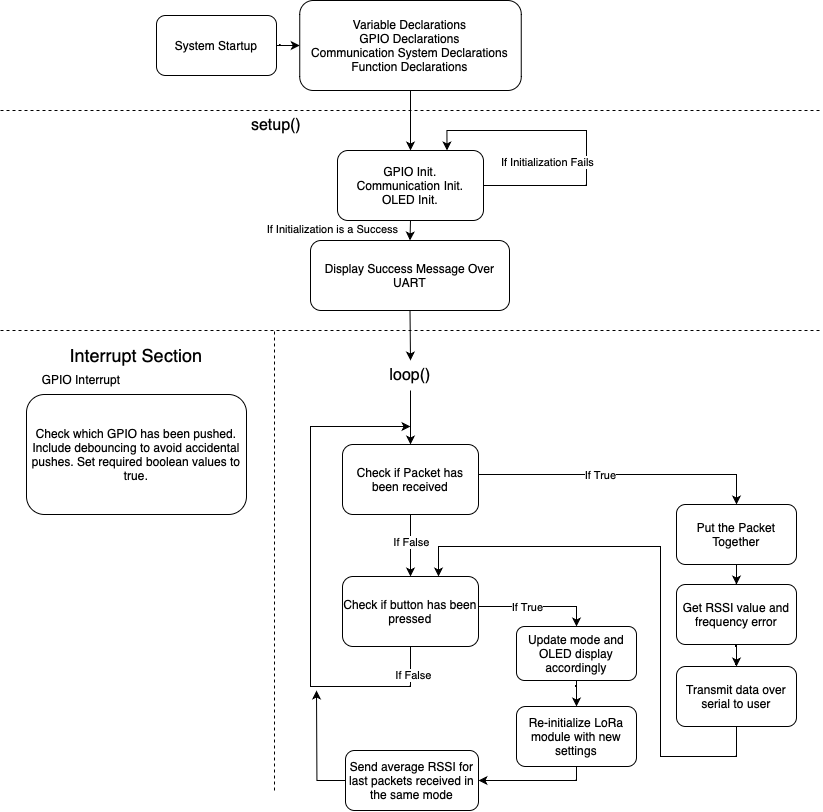
\includegraphics[width=0.7\linewidth]{../Images/receiverCircuitSoftwareFlowChart.png}
    \caption{Flow Chart of the Receiver Circuit Software}
    \label{fig:receivercircuitsoftwareflowchart}
\end{figure}

The software for the receiver was a lot simpler than for the transmitter, owing to the fact that the receiver only had to implement a LoRa module and an OLED display. Much like the transmission circuit, there is an initial setup period right after startup, where variables, functions, and GPIO pins are declared, as well as communication protocols initiated. After this initial initialization, the main loop runs. The first thing that occurs in this main loop is that a check is done to determine if a new packet of data has been received on the LoRa module.

\subsubsection{Receiver Interface with LoRa Module}
In order to interface with the LoRa module on the receiver side of things, another library was used that was designed for the Arduino coding framework, which is what my development toolchain was used for the receiver module\footnote{The LoRa library for the Arduino framework can be found \href{https://github.com/sandeepmistry/arduino-LoRa?utm_source=platformio&utm_medium=piohome}{here}.}. This library made it easy to receive packets and to determine the RSSI values associated with each packet. For interest sake, the frequency error for each received packet was also determined and printed to the user. The next step in the flow chart in figure \ref{fig:receivercircuitsoftwareflowchart} was to check whether or not a button was pressed to change the mode of the system.

\subsubsection{Handling Mode Changes}
The methodology for the detection of a button push being pressed in the receiver circuit is the exact same as in the transmitter circuit, where the push button creates a falling edge when it connects the GPIO which it is connected to through to ground, which then triggers a detection of the falling edge which causes an interrupt. The GPIOs to which the buttons are connected have pull-up resisters initiated on them. Once the buttons are pressed, and an interrupt is called, then button debouncing occurs. Once the debouncing is done, then the interrupt functions set specific booleans to true depending on which button has been pressed. This is then used in the main loop to detect the button press, and then act accordingly by changing the LoRa module settings and updating the OLED display. An effort was made towards keeping as much code out of the interrupt function as possible since it seemed to cause instability, and on the recommendation of colleagues, it was determined that using the interrupt functions to set booleans, which then trigger actions from the main loop, is a better and more stable workflow. The last thing that happens is the average RSSI value for the packets transmitted in the previous mode is sent to the user.

\section{PCB Design}
A \gls{pcb} was designed for the transmission and receiver modules, but they were both unfortunately not implemented due to design issues with the initial prototypes. Despite this, both designs can however be seen in figure \ref{fig:overallpcbdesign} below. Both PCB designs had a quick install method in mind, where the components could theoretically be transferred from the respective transmitter and receiver modules easily to their designated PCBs. All that would have to happen is some female pin headers would have to be soldered onto the PCBs themselves.

\begin{figure}[H]
    \centering
    \begin{subfigure}{0.4\textwidth}
        \centering
        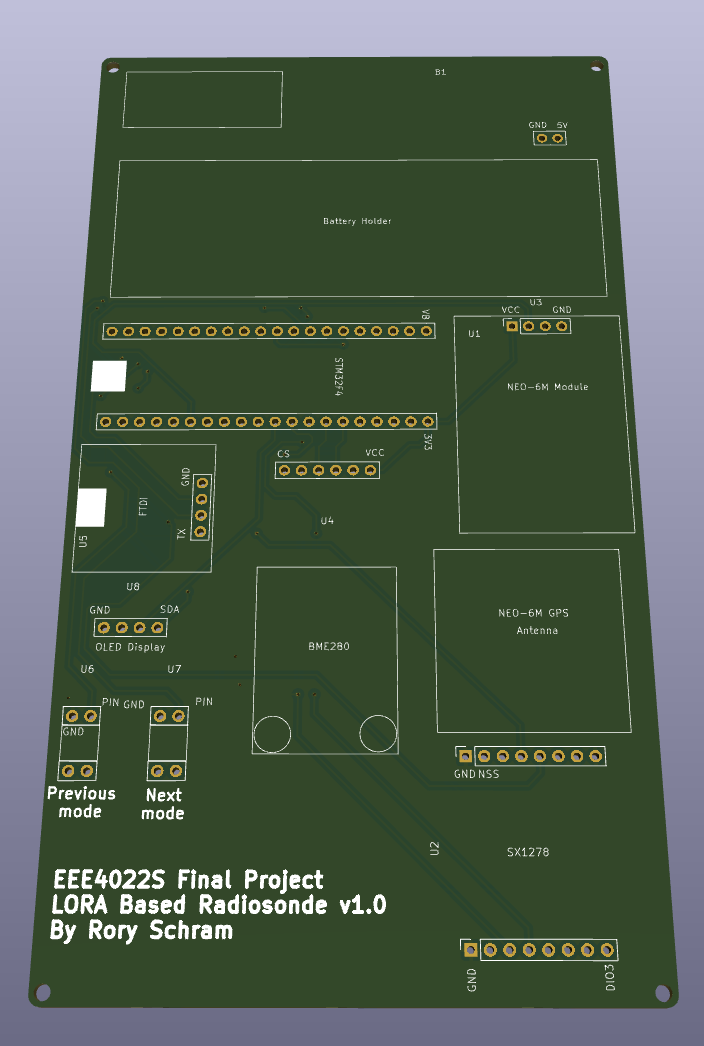
\includegraphics[width=\textwidth]{../Images/transmitterPCB.png}
        \caption{Transmitter PCB}
    \end{subfigure}\hfill
    \begin{subfigure}{0.42\textwidth}
        \centering
        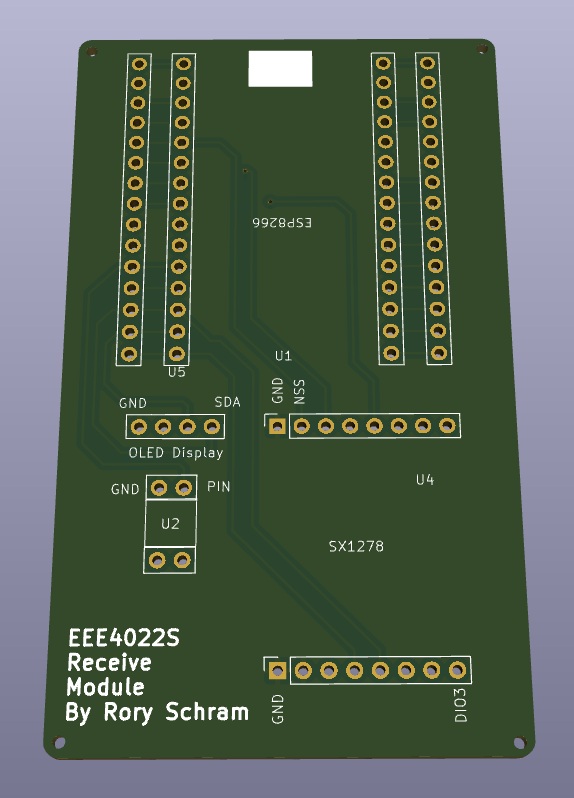
\includegraphics[width=\textwidth]{../Images/receiverPCB.png}
        \caption{Receiver PCB}
    \end{subfigure}
    \caption{PCB Design for Transmitter and Receiver}
    \label{fig:overallpcbdesign}
\end{figure}






% ----------------------------------------------------
\ifstandalone
\bibliography{../Bibliography/References}
\printnoidxglossary[type=\acronymtype,nonumberlist]
\fi
\end{document}
% ----------------------------------------------------